\documentclass[11pt]{article}

\usepackage{iftex}
\ifPDFTeX
  \usepackage[utf8]{inputenc}
  \usepackage[T1]{fontenc}
\fi
\usepackage[margin=0.92in]{geometry}
\usepackage{amsmath,amssymb,amsthm}
\usepackage{booktabs}
\usepackage{graphicx}
\usepackage{xcolor}
\usepackage{hyperref}
\usepackage{natbib}
\usepackage{microtype}
\usepackage{array}
\usepackage{multirow}
\emergencystretch=3em
\hbadness=2000

\hypersetup{
  colorlinks=true,
  linkcolor=blue,
  citecolor=blue,
  urlcolor=blue
}

\newtheorem{theorem}{Theorem}
\newtheorem{proposition}{Proposition}
\newtheorem{assumption}{Assumption}

\title{\textbf{Collision-Zone Feature Acquisition: Threshold-Aware Discovery and Residual Learning for Clinical Prediction}}

\author{
  Wayne A. Satz, MD$^*$\\
  \small Department of Emergency Medicine, Lewis Katz School of Medicine at Temple University,\\
  \small Philadelphia, PA 19140, USA\\
  \small $^*$Correspondence: \texttt{satzwa@temple.edu} \quad|\quad Preprint Version: \texttt{v2.3.0} (\texttt{Preprints.org})
}

\date{November 2026}

\begin{document}

\maketitle

\begin{abstract}
In imbalanced clinical prediction, diagnostic features that improve global probability estimation across abundant low-risk encounters may contribute little to decisions near a clinical action threshold. Building on established threshold-tailored Beta proper scoring rules, we develop a threshold-aware feature acquisition framework in which a shared Beta--Kullback--Leibler geometry coordinates channel discovery, stratified pilot sampling, localized residual learning, and Value-of-Information panel routing while retaining a globally trained prediction model. Across $1{,}000$ synthetic dilution replicates, threshold-aware discovery recovered the decision-relevant feature in $80.5\%$ of replicates versus $8.3\%$ for global conditional mutual information, and outperformed direct fixed-threshold utility optimization in factorial benchmarks ($64.7\%$ vs.\ $47.7\%$ recovery; $p_{\text{DH}}=0.0006$). Across $600{,}154$ retrospective encounters from five hospitals with explicit patient-level procedure and assay costing, common-panel bagged routing yielded $+5.77$ versus $+4.70$ Net Benefit per $1{,}000$ on external Emory $6\text{h}$-summary intensive-care sepsis evaluations ($\Delta\text{NB}=+1.07$, $95\%$ CI $[-0.18, +2.32]$, $p_{\text{DH}}=0.094$) and matched global selection on single-draw point-in-time lactate ($+5.02$ vs.\ $+5.12$). On previously untested cross-campus emergency department transfer ($N=71{,}706$), the framework improved utility in low-acuity visits ($+0.50/1{,}000$, $p_{\text{DH}}=0.0022$) and all-comers ($+0.23/1{,}000$, $p_{\text{DH}}=0.0412$). Advantages concentrate when subthreshold decoys compete for finite budgets; observational assay availability, calibration shift, and cost sensitivity constrain prospective deployment.
\end{abstract}

\vspace{4pt}
\noindent\textbf{Keywords:} Biomedical informatics methodology; active feature acquisition; proper scoring rules; two-phase stratified sampling; Value of Information; Decision Curve Analysis; calibration; clinical decision support.

\section{Introduction and the Decision-Information Dilution Hypothesis}
\label{sec:intro}

In acute-care clinical prediction---such as intensive care unit (ICU) sepsis surveillance \citep{singer2016sepsis3,reyna2020early} and inpatient admission triage among low-acuity emergency department (ED) arrivals \citep{hong2018predicting}---most encounters have predicted risks substantially below the clinical action threshold $\tau^* = C_{\text{FP}} / (C_{\text{FP}} + C_{\text{FN}})$ \citep{vickers2006decision,kerr2016assessing}. When routine bedside covariates $X_{\text{base}}$ leave diagnostic ambiguity near $\tau^*$, clinicians or automated workflows may acquire costly Stage-2 information channels $Z_1, \dots, Z_M$, such as laboratory assay panels or outside health-information-exchange (HIE) modules \citep{turney1995cost,saartsechansky2009active,bilgic2011value,covert2023learning,vonkleist2025evaluation}. Unlike class-reweighting or synthetic oversampling heuristics that distort probability calibration without adding information \citep{chawla2002smote,elkan2001foundations,vancalster2019calibration,vandengoorbergh2022harm}, cost-sensitive feature acquisition can genuinely resolve clinical uncertainty---provided the acquired features alter decisions across $\tau^*$.

Conventional information-theoretic feature discovery and dynamic active feature acquisition (AFA; \citealp{covert2023learning}) rank candidate channels by conditional mutual information (expected Shannon log-loss reduction). Under \citet{schervish1989general}'s integral representation of strictly proper scoring rules \citep{buja2005loss,gneiting2007strictly}, log-loss averages cost-weighted classification losses with threshold density $w_{\log}(\tau) = [\tau(1-\tau)]^{-1}$. Although divergent probability-scale curvature as $p \to 0^+$ does not force proportional updates to have divergent information gain---for example, updating $p \to 1.5p$ yields exact Bernoulli Kullback--Leibler (KL) divergence $D_{\text{KL}}(1.5p \,\|\, p) = O(p) \to 0$ ($1.09 \times 10^{-3}$, $1.08 \times 10^{-4}$, and $1.08 \times 10^{-5}$ at $p = 1\%$, $0.1\%$, and $0.01\%$)---it weights subthreshold risk variation heavily relative to threshold-focused alternatives whenever baseline discrimination places a large fraction of the population well below $\tau^*$. This motivates our central testable hypothesis:
\begin{quote}
\textbf{Decision-Information Dilution Hypothesis:} \emph{Under finite discovery or testing budgets and heterogeneous risk distributions, features that explain substantial variation among abundant subthreshold encounters can dominate global information rankings despite rarely moving posterior probabilities across $\tau^*$. Coordinating feature valuation, pilot sampling, and localized residual learning around $\tau^*$ recovers decision-relevant tie-breakers when subthreshold decoys compete, whereas conventional global learning suffices when Stage-2 features act homogeneously without competing decoys.}
\end{quote}

\subsection{Relationship to Prior Literature and Methodological Contributions}

Threshold-tailored proper scoring rules and decision-theoretic feature acquisition each have rich foundations. \citet{buja2005loss} established the Beta family of strictly proper binary scoring rules, analyzed the boundary curvature of log-loss, and derived mode-aligned parameterization $\tau^* = (\alpha - 1)/(\alpha + \beta - 2)$ (their Section~12, Eq.~38) to concentrate probability loss around a misclassification-cost threshold. Early cost-sensitive learning \citep{turney1995cost}, expected-utility active feature-value acquisition \citep{saartsechansky2009active}, and subset-level Value of Information lattices (\texttt{VOILA}; \citealp{bilgic2011value}) connected feature costs directly to classification risk, while \citet{covert2023learning} modernized greedy conditional mutual information (CMI) policies and \citet{vonkleist2025evaluation} formalized causal and missing-data assumptions for evaluating AFA on observational time-varying clinical records.

Rather than claiming priority for threshold-weighted Beta scoring or decision-theoretic acquisition individually, our contribution is an \emph{integrated statistical architecture} (\texttt{collision-zone-ed}) organized around a single shared threshold geometry:
\begin{enumerate}
  \item \textbf{Unified Beta--KL Threshold Geometry Across Discovery, Pilot Sampling, and Residual Learning (Section~\ref{sec:methods}, Proposition~\ref{prop:unification}):} Building on \citet{buja2005loss}'s mode-aligned $\operatorname{Beta}(1+\kappa\tau^*, 1+\kappa(1-\tau^*))$ proper score $S_{\tau^*,\kappa}$, we exploit the exact algebraic identity equating its peak-normalized threshold density to the Boltzmann Bernoulli KL gate $\exp(-\kappa D_{\text{KL}}(\operatorname{Bern}(\tau^*)\|\operatorname{Bern}(p)))$. This shared kernel aligns Stage-A channel valuation, High-Signal False Positive Neyman pilot allocation \citep{horvitz1952generalization,lumley2010complex,tao2020optimal}, and Stage-2 KL-gated residual boosting without downweighting global training data.
  \item \textbf{Decisive Factorial Comparison Against Direct Decision-Utility Objectives and Regime Mapping (Sections~\ref{sec:res_sim}--\ref{sec:res_sepsis}):} Across controlled $6\times 2$ synthetic and $5\times 3$ clinical discovery-by-backbone factorials, we test why smooth strictly proper Beta valuation outperforms discontinuous fixed-threshold empirical utility in finite pilots, and map a $36$-cell simulation design ($1{,}440$ runs) characterizing when threshold-aware acquisition outperforms versus ties global CMI.
  \item \textbf{Patient-Level Panel-Cost Ledger and Observational Evaluation Governance Across $600{,}154$ Encounters (Sections~\ref{sec:study_design}--\ref{sec:discussion}):} We price specimen-collection procedures alongside per-assay CPT fees, distinguish single-draw point-in-time laboratory specimens from multi-hour EHR summary retrieval, evaluate locked common-panel ensembles across BIDMC $\to$ Emory ICU sepsis and multi-campus Yale ED triage (including previously untested Campus C, $N=71{,}706$), and audit Fixed-Horizon vs.\ Remaining-Stay timing, unlabeled vs.\ historical prior-shift adaptation \citep{saerens2002adjusting}, clinician-ordering observability \citep{agniel2018biases,vonkleist2025evaluation}, and repeated-sampling conformal alerting \citep{jin2023selection}.
\end{enumerate}

\section{Unified Threshold-Aware Methodology}
\label{sec:methods}

Let $(X_{\text{base}}, Z_1, \dots, Z_M, Y) \sim \mathbb{P}$ denote an encounter with zero-marginal-cost intake predictors $X_{\text{base}} \in \mathcal{X}$, $M$ candidate Stage-2 channels $Z_m \in \mathcal{Z}_m$ with discovery unit weights $c_m > 0$ (discovery budget $\sum_{m \in \mathcal{S}} c_m \le B$), and binary outcome $Y \in \{0,1\}$. A clinical decision contract $\mathcal{K} = (C_{\text{FP}}, C_{\text{FN}}, q_{\text{target}})$ defines the rational Bayes action threshold $\tau^* = C_{\text{FP}} / (C_{\text{FP}} + C_{\text{FN}}) \in (0, 1)$. At deployment, if an encounter acquires channel subset $A_i \subseteq \{1,\dots,M\}$, it incurs an explicit patient-level acquisition cost $C_i(A_i)$ (expressed in $C_{\text{FP}}$ units) decomposing specimen/retrieval procedure overhead and per-channel processing fees:
\begin{equation}
  C_i(A_i) = \mathbb{I}\{A_i \ne \emptyset\}\, c_{\text{proc}}(A_i) + \sum_{m \in A_i} c_{\text{assay}, m},
  \label{eq:cost_ledger}
\end{equation}
where in venous/arterial bloodwork $c_{\text{proc}}(A_i) = c_{\text{venipuncture}} + c_{\text{ABG}}\mathbb{I}\{\text{ABG} \in A_i\}$. Following \citet{vickers2006decision} and \citet{kerr2016assessing}, Net Benefit per $1{,}000$ encounters ($\operatorname{NB}_{1000}$) and prevalence-normalized Standardized Net Benefit ($\operatorname{sNB} = \operatorname{NB}_{1000}/(1000\pi)$) for routed risk predictions $\hat{p}_{\text{route},i}$ are
\begin{equation}
  \operatorname{NB}_{1000} = \frac{1000}{N_{\text{test}}} \sum_{i=1}^{N_{\text{test}}} \left[ \mathbb{I}\{\hat{p}_{\text{route},i} \ge \tau^*, Y_i = 1\} - \frac{\tau^*}{1-\tau^*} \mathbb{I}\{\hat{p}_{\text{route},i} \ge \tau^*, Y_i = 0\} - \frac{C_i(A_i)}{C_{\text{FN}}} \right].
  \label{eq:nb_ledger}
\end{equation}
Formal mathematical statements, regularity conditions, counterexamples, and proofs appear in Appendix~\ref{app:proofs}.

\subsection{Shared Beta--KL Threshold Geometry}
\label{sec:geometry}

Following \citet{schervish1989general} and \citet{buja2005loss}, replacing $w_{\log}(\tau) = [\tau(1-\tau)]^{-1}$ with a mode-centered $\operatorname{Beta}(\alpha, \beta)$ threshold density parameterized by $\alpha = 1 + \kappa\tau^*$ and $\beta = 1 + \kappa(1 - \tau^*)$ ($\kappa > 0$) yields the closed-form strictly proper score $S_{\tau^*,\kappa}(y,p)$ in Appendix Eq.~\eqref{eq:schervish_closed}. Crucially, dividing $w_{\tau^*,\kappa}(p) = p^{\kappa\tau^*}(1-p)^{\kappa(1-\tau^*)}/B(\alpha,\beta)$ by its unique maximum at $p = \tau^*$ reveals an exact algebraic equivalence with the Bernoulli KL Boltzmann gate:
\begin{equation}
  \frac{w_{\tau^*,\kappa}(p)}{w_{\tau^*,\kappa}(\tau^*)} = \left(\frac{p}{\tau^*}\right)^{\kappa\tau^*}\left(\frac{1-p}{1-\tau^*}\right)^{\kappa(1-\tau^*)} = \exp\!\Big(-\kappa\, D_{\text{KL}}\big(\operatorname{Bern}(\tau^*) \,\|\, \operatorname{Bern}(p)\big)\Big) \equiv \pi_{\kappa}(p).
  \label{eq:beta_kl_identity}
\end{equation}
As illustrated in Figure~\ref{fig:fig1}A (verified numerically to $< 6 \times 10^{-15}$ across $(\tau^*,\kappa)$), the normalized Beta proper-score weight and the KL gate coincide identically. Moreover, subthreshold curvature suppression scales with the dimensionless product $\kappa\tau^*$, creating an empirical trade-off against active collision sample mass $M(\kappa) = \sum_{i=1}^N \pi_{\kappa}(\hat{p}_{1,i})^2$ (Figure~\ref{fig:fig1}B); bisecting $\kappa^* \in [0, \kappa_{\max}]$ subject to $M(\kappa^*) \ge M_{\min}$ adapts kernel sharpness automatically across clinical thresholds.

\begin{figure}[t!]
\centering
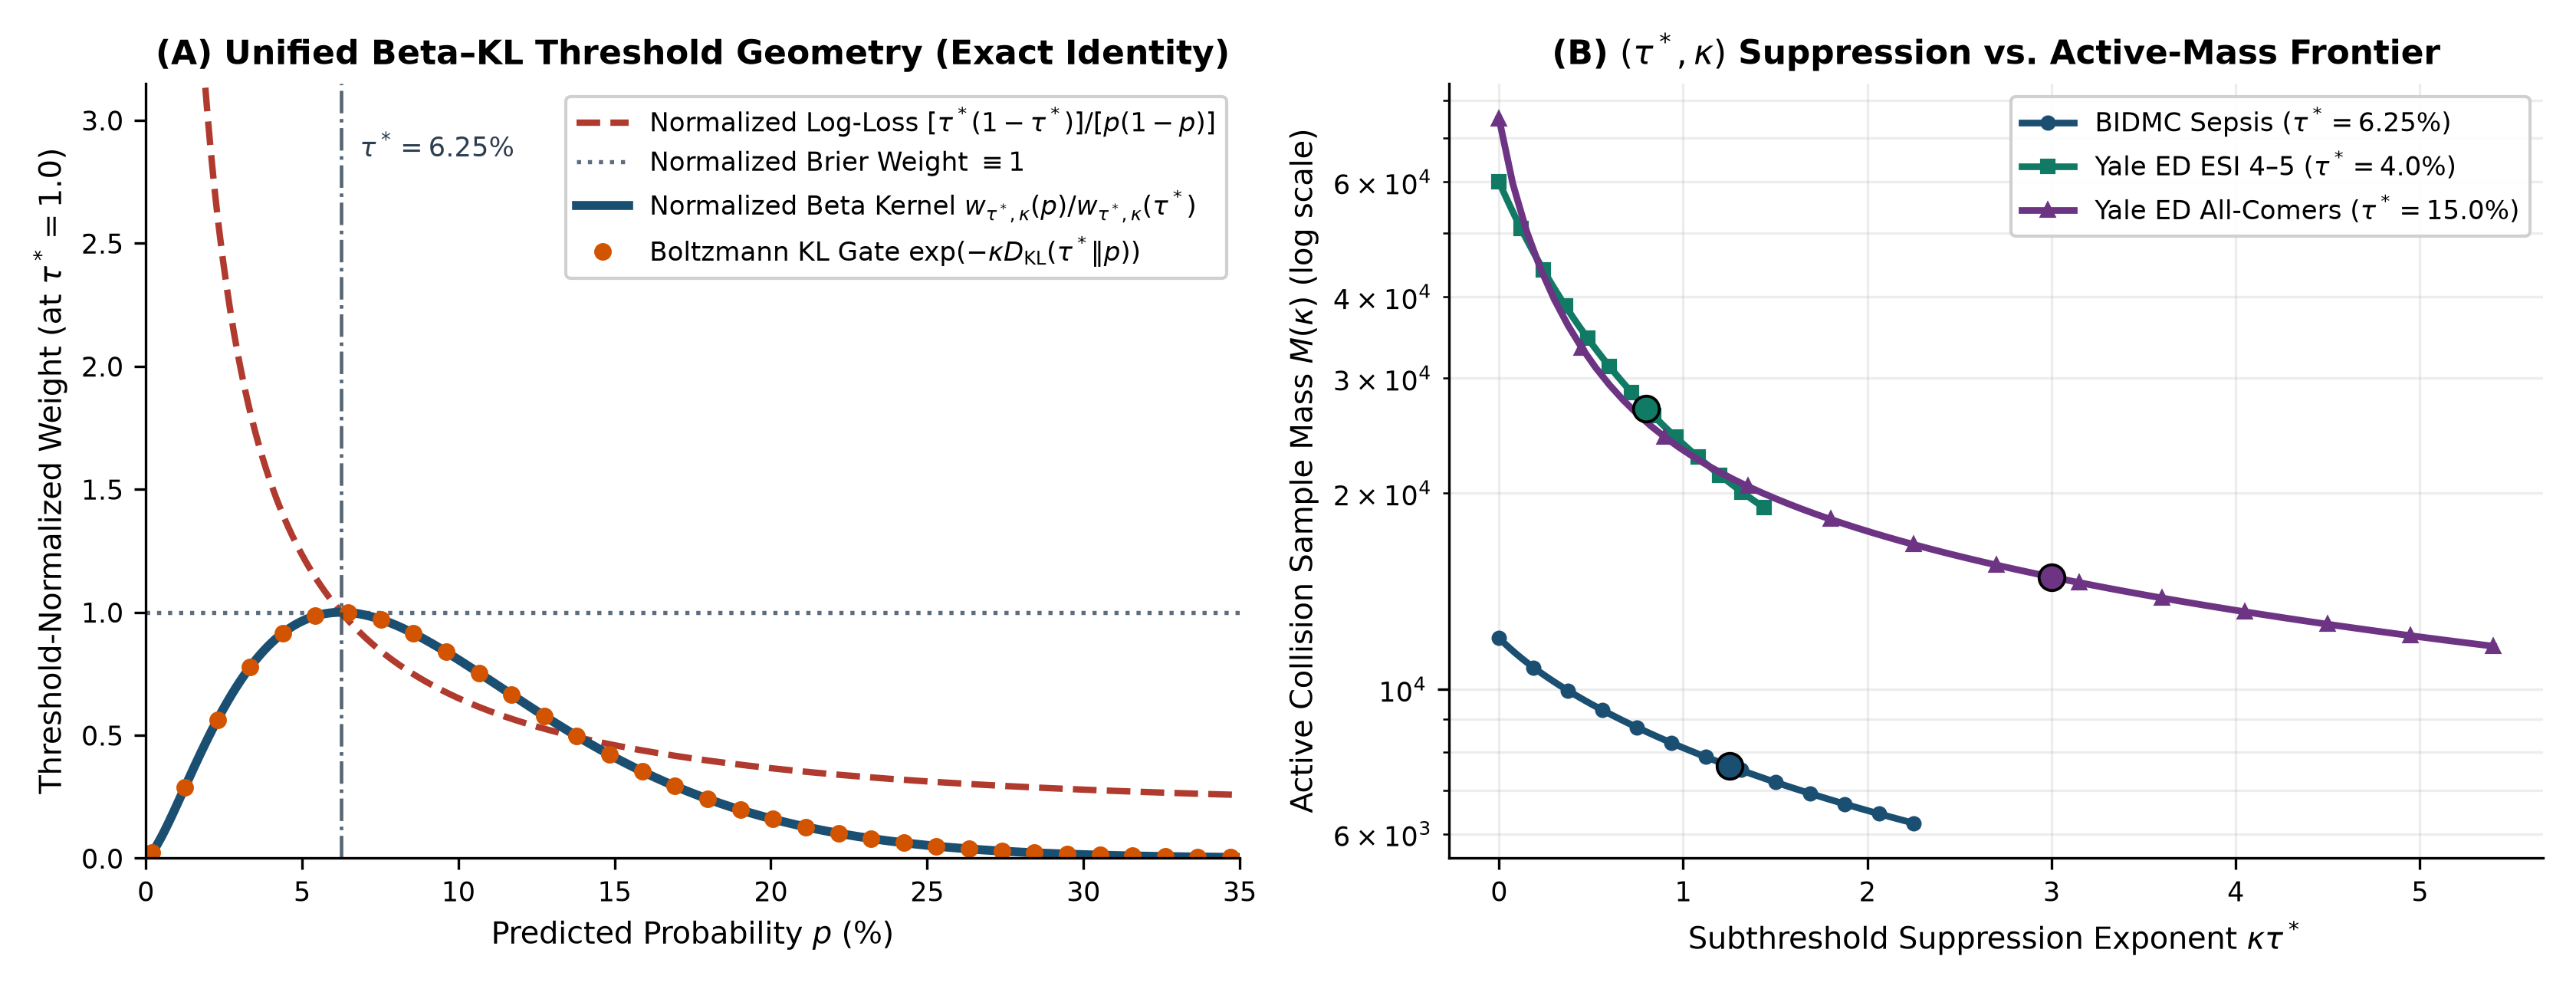
\includegraphics[width=0.98\textwidth]{fig1_unified_geometry_and_frontier.png}
\caption{Unified Beta--KL threshold geometry and $(\tau^*,\kappa)$ active-mass frontier. \textbf{(A)} Exact coincidence between the peak-normalized Beta proper-score density $w_{\tau^*,\kappa}(p)/w_{\tau^*,\kappa}(\tau^*)$ \citep{buja2005loss} and the Boltzmann Bernoulli KL gate $\exp(-\kappa D_{\text{KL}}(\operatorname{Bern}(\tau^*)\|\operatorname{Bern}(p)))$ at $\tau^*=6.25\%, \kappa=24$, contrasted against normalized log-loss curvature and constant Brier weighting. \textbf{(B)} Empirical $(\tau^*,\kappa)$ frontier of active collision sample mass $M(\kappa)$ versus suppression exponent $\kappa\tau^*$ across three cohorts ($\kappa^*$ marked).}
\label{fig:fig1}
\end{figure}

\subsection{Stage-A Stratified Pilot Discovery and Inferential Scope}
\label{sec:stage_a}

Out-of-fold (OOF) Platt-calibrated Stage-1 predictions $\hat{p}_{1,i}$ \citep{platt1999probabilistic} partition $\mathcal{D}_{\text{train}}$ ($N$ rows) into $H \le 2 B_{\text{score}}$ strata $(Y_i, b_i)$ across $B_{\text{score}}=8$ quantile bins of $\operatorname{logit}(\hat{p}_1)$. Constrained Neyman allocation \citep{lumley2010complex,tao2020optimal} draws a without-replacement Phase-2 pilot $\mathcal{P}$ ($n_{\text{pilot}} = \lfloor \rho N \rceil$, Horvitz--Thompson weights $w_i = N_{h(i)}/n_{h(i)}$) concentrated on \emph{High-Signal False Positives} ($Y_i=0, \hat{p}_{1,i} \approx \tau^*$) and boundary cases ($Y_i=1, \hat{p}_{1,i} \approx \tau^*$). Candidate channels are evaluated by Horvitz--Thompson (HT) score gain $\hat{G}_{m\mid\mathcal{S}_{t-1}} = N^{-1}\sum_{i\in\mathcal{P}} w_i \psi_{i,m\mid\mathcal{S}_{t-1}}$ using the two-phase variance estimator $\widehat{V}_{\text{total}}$ (Appendix Eq.~\eqref{eq:two_phase_var}, which uses linear HT weight $w_i r_i^2$ in $\widehat{V}_{\text{I}}$ and reduces identically to $s^2/n_{\text{pilot}}$ under simple random sampling) and Holm step-down stopping at $\alpha=0.05$ \citep{holm1979simple}.

\textbf{Hypothesis Scope and Split-Pilot Confirmation:} Adding a conditionally independent or redundant feature ($I(Y;Z\mid X)=0$) can still strictly improve a restricted finite-capacity learner---for instance, $Z = X_1 \oplus X_2$ carries zero incremental population information given $(X_1,X_2)$ yet dramatically improves depth-$1$ boosted stumps (Appendix~\ref{app:proofs}). Stage-A testing therefore targets a \emph{learner-specific predictive-utility null} rather than universal biological conditional independence. Furthermore, because classical HT design-unbiasedness requires scores $\psi_i$ to be fixed with respect to Phase-2 sampling, we distinguish two protocols: (i) \textbf{Disjoint Split-Pilot Confirmation} ($\mathcal{P} = \mathcal{P}_{\text{fit}} \sqcup \mathcal{P}_{\text{conf}}$), which fits candidate models strictly on $\mathcal{P}_{\text{fit}}$ so HT inference on $\mathcal{P}_{\text{conf}}$ is conditionally exact at the cost of halving confirmation sample size; and (ii) \textbf{$4$-Fold Cross-Fitted Discovery} on $\mathcal{P}$, which maximizes finite-pilot recovery power and functions as an empirically conservative discovery rule validated across six stress scenarios (Section~\ref{sec:res_sim}).

\subsection{Stage-2 KL-Gated Residual Learning and Threshold-Crossing VOI Routing}
\label{sec:stage_b}

To localize model corrections near $\tau^*$ without downweighting training rows or starving tree leaves, we retain unweighted Bernoulli log-likelihood and combine a $100\%$-sample global LightGBM backbone $f_{\text{glob}}(x,z)$ \citep{ke2017lightgbm} with a residual specialist $\Delta_{\text{CZ}}$ modulated by the probabilistic-OR union gate $\pi_{\text{union}}(\ell_1, f_{\text{glob}}) = 1 - (1 - \pi_{\kappa^*}(\sigma(\ell_1)))(1 - \pi_{\kappa^*}(\sigma(f_{\text{glob}}))) \in (0,1]$:
\begin{equation}
  f(x, z) = \alpha_0 + \beta_{\text{glob}}\, f_{\text{glob}}(x, z) + \beta_{\text{CZ}}\, \pi_{\text{union}}\!\big(\ell_1(x), f_{\text{glob}}(x, z)\big)\, \Delta_{\text{CZ}}\!\big(\ell_1(x), f_{\text{glob}}(x, z), z_{\mathcal{S}}\big),
  \label{eq:fluid_decomp}
\end{equation}
stacked strictly via $3$-fold OOF predictions on $\mathcal{D}_{\text{train}}$ \citep{wolpert1992stacked,vanderlaan2007super} so $\mathcal{D}_{\text{cal}}$ remains exchangeable. Because raw $\hat{\beta}_{\text{CZ}}$ is not invariant to joint rescaling $(\Delta' = a\Delta, \beta' = \beta/a)$, we quantify actual specialist intervention via the scale-invariant root-mean-square (RMS) gated log-odds contribution $R_{\text{CZ}} = [N^{-1}\sum_{i=1}^N (\hat{\beta}_{\text{CZ}}\pi_{\text{union},i}\Delta_{\text{CZ},i})^2]^{1/2}$ and the fraction of threshold decisions flipped relative to the global backbone.

At deployment, writing Bayes point risk as $L^*(p) = \min\{p C_{\text{FN}}, (1-p)C_{\text{FP}}\} = C_{\text{FN}}p - (C_{\text{FN}}+C_{\text{FP}})(p-\tau^*)_+$, any mean-preserving posterior update $\mathbb{E}[P_2 \mid X_{\text{base}}=x] = P_1(x)$ satisfies the exact \emph{threshold-crossing Value-of-Information identity}:
\begin{equation}
  \operatorname{VOI}(x) = (C_{\text{FN}} + C_{\text{FP}})\Big(\mathbb{E}\big[(P_2 - \tau^*)_+ \mid X_{\text{base}}=x\big] - \big(P_1(x) - \tau^*\big)_+\Big) \ge 0,
  \label{eq:voi_crossing}
\end{equation}
where $(u)_+ = \max(u,0)$. Thus a panel has positive Bayes decision value if and only if its posterior distribution crosses $\tau^*$ with nonzero probability. Our default \emph{Empirical Martingale VOI} centers $K=33$ empirical $\mathcal{D}_{\text{cal}}$ log-odds quantiles $\{\delta_{b(p_1),r}\}_{r=1}^K$ via the unique offset $\mu^*(p_1)$ enforcing $K^{-1}\sum_{r=1}^K \tilde{P}_{2,r} = p_1$, triggering acquisition of the locked panel $\mathcal{S}_{\text{common}}$ whenever $\widehat{\operatorname{VOI}}_{\text{emp}}(p_1) > C(\mathcal{S}_{\text{common}})$. While martingale centering guarantees nonnegativity under the constructed distribution, deployment accuracy depends on how well the empirical conditional update distribution matches true Stage-2 heterogeneity, which we benchmark directly against covariate-enriched martingale VOI, uncentered VOI, direct Bayes-risk regression, distance-to-threshold, and Shannon entropy.

\section{Experimental Design, Estimands, and Provenance}
\label{sec:study_design}

We evaluate synthetic experiments and five retrospective hospital cohorts ($600{,}154$ encounters total):
\begin{enumerate}
  \item \textbf{Synthetic Suites (Section~\ref{sec:res_sim}):} (i) $1{,}000$-replicate dilution benchmark ($N=10{,}000, \tau^*=10\%, 94\%$ subthreshold) and $3\times 15$ leaf-starvation benchmark; (ii) $6$-scenario FWER/power stress suite ($200$ replicates/scenario: correlated nulls $r=0.70$, nonlinear baseline echoes, weak signals, suppressors, unequal channel costs, and pairwise synergy) comparing cross-fitted discovery against disjoint $50/50$ split-pilot confirmation; (iii) decisive $6$-objective $\times$ $2$-backbone discovery factorial ($300$ replicates, $N=8{,}000$); (iv) $200$-replicate quadrature Oracle VOI calibration audit; and (v) a $36$-cell fractional-factorial regime map ($40$ replicates/cell $= 1{,}440$ runs) crossing collision mass ($4\%, 12\%, 25\%$), subthreshold decoy strength ($0.0, 0.95, 1.45$), feature heterogeneity, and threshold-to-prevalence ratio.
  \item \textbf{Multicenter ICU Sepsis Benchmarks (\citealp{goldberger2000physionet,reyna2020early}; BIDMC $\to$ Emory, Section~\ref{sec:res_sepsis}):} Stage-1 uses $49$ bedside vital-sign/demographic summaries at $\tau^*=6.25\%$ ($C_{\text{FN}}/C_{\text{FP}}=15, B=3.2, 20\%$ pilot). Under \texttt{PanelCostSchedule} ($c_{\text{venipuncture}}=0.010, c_{\text{ABG}}=0.010$, CPT assay scale $0.020$; \citealp{cms2025clfs}), a single venous \texttt{Lactate} draw costs $0.010 + 0.020(1.00) = 0.030\,C_{\text{FP}}$, matching legacy single-assay scaling while pricing multi-assay panels and arterial blood gases ($0.0558$ alone; $0.0758$ with venous lactate) explicitly. To separate new specimen ordering from EHR trajectory review, we evaluate \textbf{both} \emph{Single-Draw Point-in-Time Specimens} (\texttt{\_last} assay value only) and \emph{First-$6\text{h}$ Trajectory Summaries} (\texttt{\_last, \_min, \_max}) on Measured-Bloodwork Track B1b ($N_{\text{BIDMC}}=8{,}345 \to N_{\text{Emory}}=6{,}463, 349$ events), alongside All-Comers Track A ($19{,}972 \to 19{,}696$), \texttt{AgnielDeconfounder} Track B1a, $4\text{h}+2\text{h}$-gap prior-shift Track B2, a $16$-cell $4/6/8/12\text{h} \times \{\text{next }2\text{h}, 6\text{h}, 12\text{h}, \text{remaining stay}\}$ matrix, and SOFA incorporation-bias exclusions.
  \item \textbf{Multi-Campus Yale ED Admission Benchmarks (\citealp{hong2018predicting}; $560{,}486$ Visits Across Campuses A, B, and C, Section~\ref{sec:res_yale}):} Stage-2 comprises $M=18$ longitudinal EHR/HIE record-retrieval modules ($B=3.0$) priced via connection plus per-module retrieval overhead ($0.005 + 0.010\sum c_m$ on low-acuity \texttt{ESI 4--5}, $\tau^*=4.0\%, C_{\text{FN}}/C_{\text{FP}}=24$; $0.004 + 0.008\sum c_m$ on all-comers, $\tau^*=15.0\%$). Beyond Campus A ($322{,}283$) $\to$ Campus B ($166{,}497$ all-comers; $51{,}205$ \texttt{ESI 4--5}), we evaluate frozen Campus A common-panel models zero-shot on \textbf{Campus C} ($N=71{,}706$ all-comers, $15.62\%$ admission; $N=31{,}430$ \texttt{ESI 4--5}, $1.96\%$ admission), which had never previously served as a cross-campus transfer target (though included in pooled within-system reference runs). Direct audit of \citet{hong2018predicting}'s de-identified archive confirms that \texttt{pat\_mrn\_id} indexes $560{,}486$ unique encounters rather than longitudinal repeat patients; all Yale splits are therefore encounter- or campus-level.
\end{enumerate}

\textbf{Deployment Estimands and Inferential Protocol:} Across $R$ source training splits, averaging split predictions before thresholding is not algebraically equivalent to averaging single-policy decisions ($\mathbb{I}\{R^{-1}\sum_r p_i^{(r)} \ge \tau^*\} \ne R^{-1}\sum_r \mathbb{I}\{p_i^{(r)} \ge \tau^*\}$), nor can an ensemble bill a single assay fee if constituent splits require distinct panels. We therefore separate four explicit estimands:
\begin{enumerate}
  \item \textbf{Common-Panel Bagged VOI (Primary Deployable Estimator):} Locks a single panel $\mathcal{S}_{\text{common}}$ discovered on the source hospital, trains all $R$ ensemble members strictly on $\mathcal{S}_{\text{common}}$, issues one binary query $Q_i^{\text{bag}} = \mathbb{I}\{\widehat{\operatorname{VOI}}_{\text{bag}}(\bar{p}_{1,i}) > C(\mathcal{S}_{\text{common}})\} \in \{0,1\}$, and bills exact $C(\mathcal{S}_{\text{common}})Q_i^{\text{bag}}$. Every Stage-2 prediction uses only features recorded in that encounter's billed ledger.
  \item \textbf{Union-Panel Bagged VOI (Diagnostic):} Retains heterogeneous per-split panels $\mathcal{S}^{(1)}, \dots, \mathcal{S}^{(R)}$ and bills the full union fee $C\big(\bigcup_{r=1}^R \mathcal{S}^{(r)}\big)$ whenever $Q_i^{\text{bag}}=1$.
  \item \textbf{Mean Single-Split Policy Utility (\texttt{Per-Split}):} Mean retrospective utility across $r=1,\dots,R$ of $\operatorname{NB}\big(Y, \hat{p}^{(r)}, C(\mathcal{S}^{(r)})Q^{(r)}\big)$ when deploying one randomly selected source-trained policy.
  \item \textbf{Fractionally Billed Probability-Averaged Ensemble (\texttt{Frac.\ Ens.}):} Thresholds $\bar{p}_i = R^{-1}\sum_r \hat{p}_{\text{route},i}^{(r)}$ and bills $R^{-1}\sum_r C(\mathcal{S}^{(r)})Q_i^{(r)}$, reported solely as a continuous benchmark without Rao--Blackwellization claims.
\end{enumerate}
Domain Minimum Clinically Important Differences (\texttt{MCID}) are $1.0/1{,}000$ for ICU sepsis, $0.25/1{,}000$ for \texttt{ESI 4--5}, and $0.40/1{,}000$ for ED all-comers. Paired patient-level multinomial bootstraps ($B=10{,}000$ for cohort contrasts; $B=5{,}000$ for subgroups) provide $95\%$ percentile CIs and two-sided Davison--Hinkley empirical sign-tail probabilities $p_{\text{DH}} = 2(\min(k_-,k_+)+1)/(B+1)$ \citep{davison1997bootstrap} conditional on the fitted policies and observed target cohort. Core algorithmic constants were committed in \texttt{8c8c4c8} (\texttt{2026-11-22}); all \texttt{v2.3.0} panel-ledger, factorial, horizon, and Campus C evaluations are explicitly documented as post-review methodological repairs (Appendix~\ref{app:sensitivity}; code commit \texttt{5362988}, $50/50$ \texttt{pytest} tests passing).

\section{Results}
\label{sec:results}

\subsection{Synthetic Discovery Factorials, Stress FWER, VOI Calibration, and Regime Boundaries}
\label{sec:res_sim}

Table~\ref{tab:sim_factorial} and Figure~\ref{fig:fig2} summarize the synthetic suites. In the $1{,}000$-replicate dilution benchmark ($N=10{,}000, 94\%$ subthreshold), \texttt{CZ-Fluid} increases pilot High-Signal False Positive representation from $5.4\%$ (SRS) and $10.2\%$ (Global Neyman) to $19.3\%$, lifting tie-breaker recovery from $8.3\%$ ($[6.7\%, 10.2\%]$) to $\mathbf{80.5\%}$ ($[77.9\%, 82.9\%]$), holding $B=5$ sequential null FWER at $\mathbf{1.0\%}$ ($[0.5\%, 1.8\%]$; vs.\ $8.1\%$ Global-CMI) and all-null FWER at $2.6\%$, and improving Net Benefit from $+0.08$ to $\mathbf{+1.64}/1{,}000$ ($\Delta\text{NB}=+1.55$, $p_{\text{DH}}=0.0002$).

\textbf{Why Smooth Beta Scoring Beats Direct Fixed-Threshold Utility:} In the $300$-replicate $6\times 2$ discovery-by-backbone factorial ($N=8{,}000$; Table~\ref{tab:sim_factorial}, Figure~\ref{fig:fig2}A), tie-breaker recovery climbs monotonically from Global Log-Loss ($10.7\%$) to Brier ($45.3\%$), Direct Fixed-Threshold Utility ($47.7\%$), Local Band Utility ($54.0\%$), and \textbf{Beta Threshold Kernel $S_{\tau^*,\kappa}$ ($64.7\%$)}, yielding significant paired Net Benefit gains over both Direct Fixed-Threshold Utility ($\mathbf{+0.16}/1{,}000$, $95\%$ CI $[+0.07, +0.25]$, $p_{\text{DH}}=0.0006$) and Local Band Utility ($+0.13$, $[+0.06, +0.21]$, $p_{\text{DH}}=0.0004$). Because exact threshold indicators $\mathbb{I}\{\hat{p}\ge\tau^*\}$ ignore near-threshold probability movements that do not yet cross $\tau^*$ on a finite pilot, smooth strictly proper Beta weighting extracts higher signal-to-noise. Moreover, even under $100\%$ Oracle Discovery, KL-Gated Fluid Stage-2 outperforms Global Stage-2 ($+1.24$ vs.\ $+0.71/1{,}000$) by preventing subthreshold splits from diluting boundary capacity.

\begin{table}[t!]
\centering
\caption{Synthetic discovery-objective $\times$ Stage-2 backbone factorial ($300$ replicates, $N=8{,}000, \tau^*=10\%$), $6$-scenario FWER stress suite ($200$ replicates/scenario), and quadrature Oracle VOI routing audit ($200$ replicates). Proportions show exact Clopper--Pearson $95\%$ CIs.}
\label{tab:sim_factorial}
\small
\resizebox{\textwidth}{!}{%
\begin{tabular}{llcccc}
\toprule
\textbf{Suite / Arm} & \textbf{Comparator / Scenario} & \textbf{Tie-Breaker Recovery} & \textbf{Decoy Hijack / Null FWER} & \textbf{Global S2 NB $/1\text{k}$} & \textbf{KL-Gated Fluid S2 NB $/1\text{k}$} \\
\midrule
\multirow{6}{*}{\shortstack[l]{\textbf{Discovery Factorial}\\($300$ reps, $N=8{,}000$;\\identical pilots \& budgets)}}
  & (A) Global Log-Loss (CMI) & $10.7\%$ ($[7.4, 14.7]$) & $82.3\%$ hijack \,|\, $11.0\%$ FWER & $-0.01 \pm 0.06$ & $+0.02 \pm 0.07$ \\
  & (B) Brier Score & $45.3\%$ ($[39.6, 51.2]$) & $1.3\%$ hijack \,|\, $1.0\%$ FWER & $+0.40 \pm 0.06$ & $+0.64 \pm 0.07$ \\
  & (D) Direct Fixed-Threshold Utility & $47.7\%$ ($[41.9, 53.5]$) & $5.3\%$ hijack \,|\, $0.7\%$ FWER & $+0.51 \pm 0.06$ & $+0.77 \pm 0.08$ \\
  & (E) Local Interval Utility & $54.0\%$ ($[48.2, 59.7]$) & $13.0\%$ hijack \,|\, $1.0\%$ FWER & $+0.48 \pm 0.07$ & $+0.81 \pm 0.08$ \\
  & \textbf{(C) Beta Kernel $S_{\tau^*,\kappa}$ (Proposed)} & $\mathbf{64.7\%}$ ($\mathbf{[59.0, 70.1]}$) & $7.0\%$ hijack \,|\, $\mathbf{2.0\%}$ \textbf{FWER} & $+0.56 \pm 0.07$ & $\mathbf{+0.94 \pm 0.08}^*$ \\
  & (F) Oracle Population Channel & $100.0\%$ (oracle) & $0.0\%$ hijack \,|\, $0.0\%$ FWER & $+0.71 \pm 0.07$ & $\mathbf{+1.24 \pm 0.08}$ \\
\midrule
\multirow{3}{*}{\shortstack[l]{\textbf{FWER Stress Suite}\\($6 \times 200$ reps, $N=6{,}000$)}}
  & Correlated Nulls ($r=0.70$) / Nonlinear Echoes & CF: $66.5\% / 67.5\%$ & \textbf{CF FWER:} $\mathbf{0.5\% / 1.0\%}$ & Split-Conf rec.: $18.5\% / 19.5\%$ & Split-Conf FWER: $2.0\% / 5.0\%$ \\
  & Unequal Costs / Pairwise Synergy & CF: $68.5\% / 38.5\%$ & \textbf{CF FWER:} $\mathbf{3.0\% / 1.0\%}$ & Split-Conf rec.: $22.0\% / 9.0\%$ & Split-Conf FWER: $3.5\% / 2.5\%$ \\
  & Suppressor / Weak Signal ($0.5\times$) & CF: $34.0\% / 5.5\%$ & \textbf{CF FWER:} $\mathbf{1.5\% / 3.0\%}$ & Split-Conf rec.: $11.0\% / 2.0\%$ & Split-Conf FWER: $1.5\% / 8.0\%$ \\
\midrule
\multirow{2}{*}{\shortstack[l]{\textbf{Oracle VOI Audit}\\($200$ reps, het.\ $\sigma(x)$)}}
  & Risk-Only Empirical Martingale VOI & $\rho_{\text{Spearman}} = 0.297 \pm 0.006$ & $\text{MAE} = 0.131$ vs.\ Oracle & Uncentered NB: $+42.40$ & \textbf{Martingale NB:} $+42.62$ (Dist.: $+41.54$) \\
  & \textbf{Covariate-Enriched Martingale VOI} & $\mathbf{\rho_{\text{Spearman}} = 0.584 \pm 0.007}$ & $\mathbf{\text{MAE} = 0.096}$ vs.\ Oracle & Direct Reg.\ NB: $+42.51$ & \textbf{Cov.-VOI NB:} $\mathbf{+43.06}$ (Oracle: $+43.39$) \\
\bottomrule
\multicolumn{6}{l}{\footnotesize $^*$Paired bootstrap $\Delta\text{NB}$ for Beta+Fluid vs.\ Direct Utility+Fluid: $+0.16$ ($[+0.07,+0.25], p_{\text{DH}}=0.0006$); vs.\ Local Utility+Fluid: $+0.13$ ($p_{\text{DH}}=0.0004$); vs.\ Global CMI: $+0.95$ ($p_{\text{DH}}=0.0002$).}
\end{tabular}%
}
\end{table}

\textbf{Stress FWER, VOI Accuracy, and the $36$-Cell Regime Map:} Across all six stress scenarios (Table~\ref{tab:sim_factorial}), $4$-fold cross-fitted Beta discovery maintains empirical sequential FWER between $0.5\%$ and $3.0\%$ while achieving $3\times$ higher step-$1$ recovery than $50/50$ split-pilot confirmation ($66.5\%\text{--}68.5\%$ vs.\ $18.5\%\text{--}22.0\%$), quantifying the finite-sample power cost of sample splitting. Under covariate-dependent Stage-2 volatility, conditioning VOI dispersion on $(p_1, X_{\text{base}})$ nearly doubles rank correlation with exact quadrature Oracle VOI ($\rho = 0.584$ vs.\ $0.297$ for risk-only binning) and approaches oracle Net Benefit ($43.06$ vs.\ $43.39$; Distance-to-Threshold $41.54$). Crucially, the $36$-cell regime map (Figure~\ref{fig:fig2}B) delineates a clear operational boundary: when subthreshold decoys are absent ($\gamma_{\text{TN}}=0$) and Stage-2 effects are homogeneous with $\tau^* > \pi$, \texttt{Global-CMI} uses full-cohort sample size efficiently and slightly outperforms \texttt{CZ-Fluid} ($\Delta\text{NB} = -0.07$ to $-0.26/1{,}000$); once subthreshold decoys compete ($\gamma_{\text{TN}} \in \{0.95, 1.45\}$), \texttt{CZ-Fluid} outperforms \texttt{Global-CMI} in $\mathbf{23/24}$ cells ($+0.17$ to $+3.75/1{,}000$).

\begin{figure}[t!]
\centering
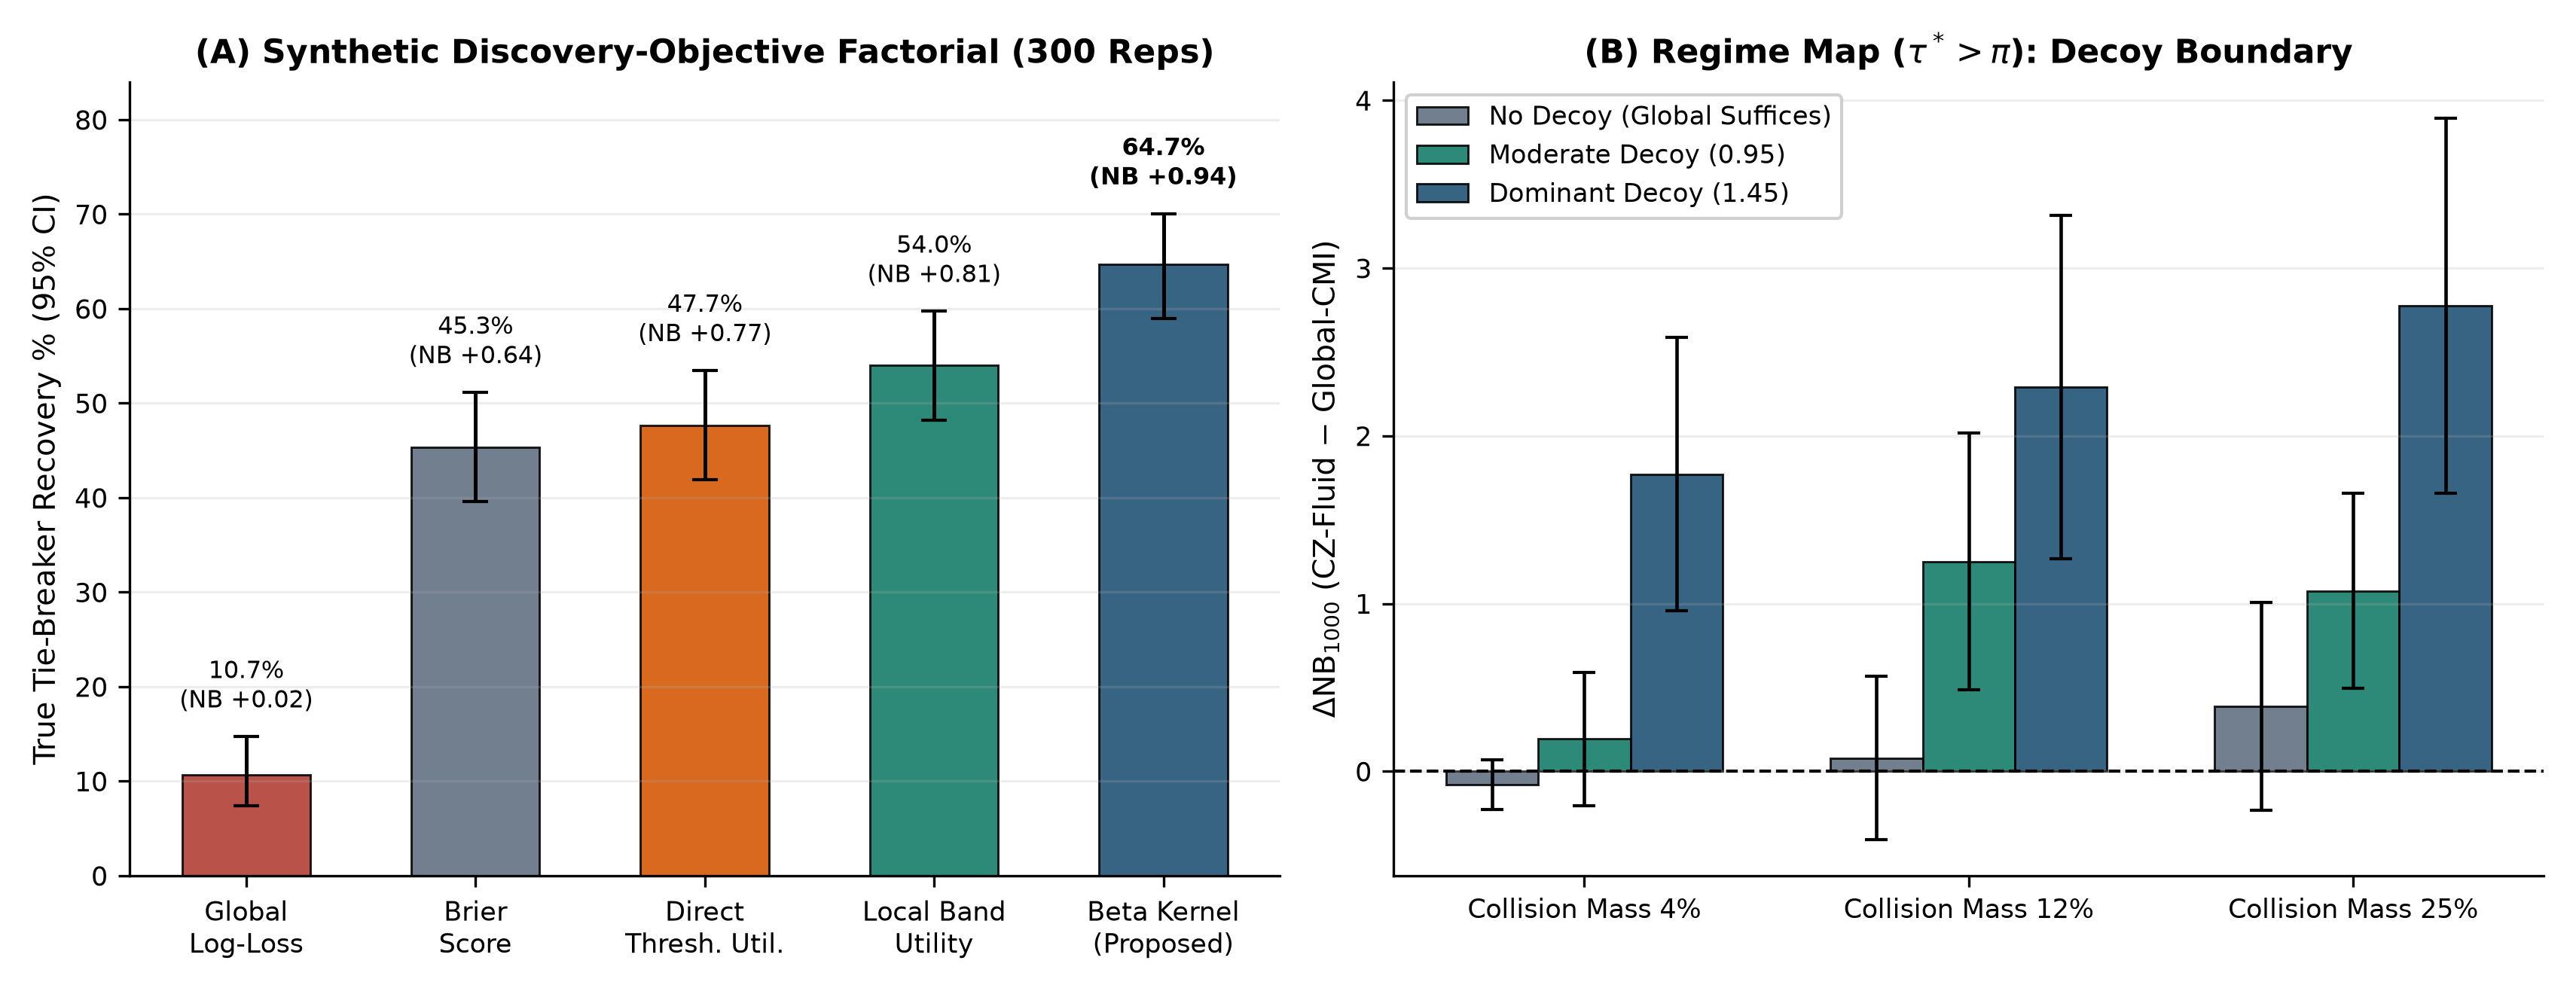
\includegraphics[width=0.98\textwidth]{fig2_synthetic_factorial_and_regime_map.png}
\caption{Synthetic discovery-objective factorial and $36$-cell regime boundary. \textbf{(A)} True tie-breaker recovery ($95\%$ Clopper--Pearson CIs) and downstream Fluid Stage-2 Net Benefit across five non-oracle discovery criteria ($300$ replicates). \textbf{(B)} $\Delta\operatorname{NB}_{1000}$ (\texttt{CZ-Fluid} minus \texttt{Global-CMI}) across collision-zone mass and subthreshold decoy strength when $\tau^* > \pi$, illustrating parity/slight global advantage without decoys and monotonic gains under decoy competition.}
\label{fig:fig2}
\end{figure}

\subsection{External ICU Sepsis Transfer Under Explicit Panel-Cost Accounting}
\label{sec:res_sepsis}

Tables~\ref{tab:sepsis_ledger}--\ref{tab:sepsis_exchange} and Figure~\ref{fig:fig3} report the repaired BIDMC $\to$ Emory sepsis evaluations ($N_{\text{ext}}=6{,}463, 349$ events, $\tau^*=6.25\%$).

\textbf{Reconciling Panel Billing and Specimen Timing:} Reproducing legacy flat-$0.03$ billing across heterogeneous per-split models yields $+4.98$ versus $+3.62/1{,}000$ ($\Delta\text{NB}=+1.36, p_{\text{DH}}=0.0428$), because $10$-split source discovery selects \texttt{lab\_lactate} only intermittently ($3/10$ CZ splits plus $1/10$ ABG; $2/10$ Global-CMI splits plus $1/10$ platelets). However, charging the $10$-split union panel ($0.0758$ vs.\ $0.0456\,C_{\text{FP}}$) reduces fixed-query utility to $+4.27$ vs.\ $+3.60$ and causes cost-rerouted VOI to abstain ($+3.43$, matching zero-query Stage-1 vitals; Figure~\ref{fig:fig3}A). Under our coherent \textbf{Common-Panel Bagged VOI} primary estimator---where full-source BIDMC discovery locks \texttt{['lab\_lactate']} ($C = 0.030\,C_{\text{FP}}$) for both \texttt{CZ-Beta} (including under $50/50$ split-confirmation on $6\text{h}$ summaries) and \texttt{Global-CMI}:
\begin{itemize}
  \item \textbf{First-$6\text{h}$ Trajectory Summaries (\texttt{\_last, \_min, \_max}):} \texttt{CZ-Fluid} achieves $\mathbf{+5.77}/1{,}000$ ($\operatorname{sNB}=10.7\%, 53.4\%$ queries; $+\mathbf{2.34}$ over Stage-1 vitals, $95\%$ CI $[+0.03, +4.63]$, $p_{\text{DH}}=0.0484$) compared with $+4.70/1{,}000$ ($47.5\%$ queries) for \texttt{Global-CMI + Global S2}. The paired difference of $\mathbf{+1.07}/1{,}000$ exceeds the prespecified $1.0/1{,}000$ \texttt{MCID} at the point-estimate level, though its $95\%$ CI ($[-0.18, +2.32]$, $p_{\text{DH}}=0.094$; $\mathbb{P}(\Delta>0)=95.3\%$) includes smaller effects and zero.
  \item \textbf{Single-Draw Point-in-Time Specimen (\texttt{\_last} Only):} When restricted to a single scalar \texttt{Lactate\_last} value reproducible by one new venipuncture, Stage-2 effects are monotone across risk strata; \texttt{CZ-Fluid} ($+5.02/1{,}000$, $R_{\text{CZ}}=0.103$) and \texttt{Global-CMI} ($+5.12/1{,}000$) perform comparably ($\Delta\text{NB} = -0.10$, $95\%$ CI $[-0.93, +0.72]$, $p_{\text{DH}}=0.822$), both improving point-estimate utility by $+1.59$ to $+1.68/1{,}000$ over Stage-1 vitals ($+3.43$, $p_{\text{DH}}=0.153$).
  \item \textbf{Clinical Discovery Factorial, Ungated Residual, and Channel-Billed AFA:} In the $5\times 3$ clinical factorial on $6\text{h}$ summaries (Table~\ref{tab:sepsis_ledger}), \textbf{Direct Fixed-Threshold Utility} and \textbf{Brier} both select $\emptyset$ ($+3.43$ NB; $+2.34$ below \texttt{CZ-Fluid}, $p_{\text{DH}}=0.057$ and $0.060$), while \textbf{Local Interval Utility} selects \texttt{lab\_glucose} ($+2.53$ NB; $\mathbf{+3.24}/1{,}000$ below \texttt{CZ-Fluid}, $95\%$ CI $[+1.06, +5.33]$, $p_{\text{DH}}=\mathbf{0.0038}$). Once clean single-panel \texttt{['lab\_lactate']} is isolated, a matched-capacity ($8$-leaf, $50$-tree) ungated residual booster achieves $+5.94$ ($6\text{h}$) and $+5.70$ (\texttt{\_last}), confirming that spatial KL gating primarily protects against multi-channel decoy interference rather than single-biomarker nonlinearity. Patient-level channel-billed \texttt{Covert-CMI} and \texttt{Direct-VOI} sequential AFA yield $+1.40$ and $+1.39$ per-split ($p_{\text{DH}}=0.0002$ below \texttt{CZ-Fluid}) and $+3.43$ and $+3.39$ under majority-mask deployment. On All-Comers Track A (\texttt{\_last}, without missingness indicators), venous \texttt{Lactate} ($C=0.030$, NB $+1.91$ Global-CMI; $+1.70$ CZ split-confirmation) outperforms arterial blood gas ($C=0.0558$, NB $+0.60$, $p_{\text{DH}}=0.0086$) once extra arterial-puncture procedure costs are billed, whereas \texttt{AgnielDeconfounder} Track B1a triggers clean $0$-channel abstention for both methods ($-1.41$).
\end{itemize}

\begin{table}[t!]
\centering
\caption{Repaired BIDMC $\to$ Emory external sepsis evaluation ($N_{\text{ext}}=6{,}463, 349$ events, $\tau^*=6.25\%, \texttt{MCID}=1.0/1{,}000$) under explicit patient-level \texttt{PanelCostSchedule} accounting ($B=10{,}000$ paired bootstraps).}
\label{tab:sepsis_ledger}
\small
\resizebox{\textwidth}{!}{%
\begin{tabular}{llccccc}
\toprule
\textbf{Channel Mode / Suite} & \textbf{Method / Factorial Arm} & \textbf{Locked / Billed Panel ($C_i$)} & \textbf{Common Bagged NB ($q\%$)} & \textbf{Per-Split Mean $\pm$ SD} & \textbf{Frac.\ Ens.\ NB} & \textbf{Paired Bootstrap Contrast ($95\%$ CI, $p_{\text{DH}}$)} \\
\midrule
\multirow{7}{*}{\shortstack[l]{\textbf{Track B1b: $6\text{h}$ Window}\\(\texttt{last, min, max} retrieval)\\$8{,}345 \to 6{,}463$}}
  & Stage-1 Bedside Vitals & $\emptyset$ ($0.000$) & $+3.43$ ($0.0\%$) & $+2.31 \pm 1.74$ & $+3.43$ & CZ vs.\ Vitals: $\mathbf{+2.34}$ ($\mathbf{[+0.03,+4.63], 0.0484}$) \\
  & Global-CMI + Global S2 & \texttt{Lactate} ($0.030$) & $+4.70$ ($47.5\%$) & $+2.83 \pm 1.88$ & $+3.48$ & Reference (Legacy flat-$0.03$: $+3.62$) \\
  & Direct Thresh.\ Util.\ + Fluid S2 & $\emptyset$ ($0.000$) & $+3.43$ ($0.0\%$) & --- & --- & CZ vs.\ Direct Util.: $+2.34$ ($[-0.07,+4.67], 0.057$) \\
  & Brier Score + Fluid S2 & $\emptyset$ ($0.000$) & $+3.43$ ($0.0\%$) & --- & --- & CZ vs.\ Brier: $+2.34$ ($[-0.08,+4.63], 0.060$) \\
  & Local Band Util.\ + Fluid S2 & \texttt{Glucose} ($0.021$) & $+2.53$ ($40.8\%$) & --- & --- & CZ vs.\ Local Util.: $\mathbf{+3.24}$ ($\mathbf{[+1.06,+5.33], 0.0038}$) \\
  & Channel-Billed AFA (CMI / VOI) & Adaptive mask $M_i$ & $+3.43 / +3.39$ (maj.) & $+1.40 / +1.39$ & --- & CZ vs.\ AFA split: $\mathbf{+4.37 / +4.39}$ ($\mathbf{0.0002}$) \\
  & \textbf{CZ-Beta + KL-Gated Fluid S2}$^\dagger$ & \texttt{Lactate} ($0.030$) & $\mathbf{+5.77}$ ($53.4\%$) & $+3.06 \pm 1.32$ & $\mathbf{+4.82}$ & vs.\ Glob: $+1.07$ ($[-0.18,+2.32], 0.094$)$^\ddagger$ \\
\midrule
\multirow{4}{*}{\shortstack[l]{\textbf{Track B1b: Single-Draw}\\(\texttt{\_last} point specimen)\\$8{,}345 \to 6{,}463$}}
  & Global-CMI + Global S2 & \texttt{Lactate\_last} ($0.030$) & $\mathbf{+5.12}$ ($45.8\%$) & $+2.60 \pm 2.26$ & $+3.43$ & Reference \\
  & Direct Util.\ / Brier + Fluid S2 & $\emptyset$ ($0.000$) & $+3.43$ ($0.0\%$) & --- & --- & CZ vs.\ Direct/Brier: $+1.59$ ($[-0.63,+3.72], 0.150$) \\
  & Channel-Billed AFA (CMI / VOI) & Adaptive mask $M_i$ & $+3.43 / +3.44$ (maj.) & $+1.50 / +1.42$ & --- & CZ vs.\ AFA split: $\mathbf{+3.53 / +3.60}$ ($\mathbf{0.0004}$) \\
  & \textbf{CZ-Beta + KL-Gated Fluid S2} & \texttt{Lactate\_last} ($0.030$) & $+5.02$ ($49.0\%$) & $\mathbf{+2.66 \pm 1.82}$ & $\mathbf{+4.33}$ & vs.\ Glob: $-0.10$ ($[-0.93,+0.72], 0.822$) \\
\bottomrule
\multicolumn{7}{l}{\footnotesize $^\dagger$Disjoint $50/50$ split-confirmation discovery selects identical \texttt{['lab\_lactate']} ($+5.77$). Matched ungated residual S2 achieves $+5.94$ ($6\text{h}$) and $+5.70$ (\texttt{\_last}).} \\
\multicolumn{7}{l}{\footnotesize $^\ddagger$Frac.\ Ens.\ $\Delta\text{NB}=+1.34$ ($[+0.20,+2.47], p_{\text{DH}}=0.0268$); $10$-split Union-Panel cost ($0.0758$ CZ vs.\ $0.0456$ Glob) yields $+4.27$ vs.\ $+3.60$ fixed-$Q$ and $+3.43$ rerouted.}
\end{tabular}%
}
\end{table}

\textbf{Clinical Exchange Triad, One-Sided Escalation, and Cost Sensitivity:} Table~\ref{tab:sepsis_exchange} reports all three operational components---sensitivity (TPs), false alerts spared (FPs), and query volume---at $\tau^*=6.25\%$. Because Stage-1 bedside vitals alert on $56.5\%$ of admissions ($249$ TPs [$71.4\%$ sensitivity], $3{,}402$ FPs), two-sided VOI routing acquires panels on $53.4\%$ of encounters ($+59.1$ queries/$1{,}000$ vs.\ \texttt{Global-CMI}) and generates utility primarily by de-escalating normolactatemic false alarms ($645$ fewer FPs vs.\ vitals and $145$ fewer FPs vs.\ \texttt{Global-CMI}, with $228$ vs.\ $230$ TPs). Implementing an explicit \textbf{Escalation-Only VOI} policy ($p_1 < \tau^*$, never de-escalating supra-threshold vitals) cuts query rate in half ($26.1\%$), eliminates all missed baseline cases, and lifts sensitivity from $71.4\%$ ($249$ TPs) to $\mathbf{76.2\%}$ ($\mathbf{266}$ \textbf{TPs}), yielding $+3.78/1{,}000$ NB ($+0.34$ over vitals) while forfeiting the false-alarm savings captured by \textbf{De-escalation-Only VOI} ($+5.43/1{,}000$ NB, $27.3\%$ queries). Across Stage-B routing comparators on $6\text{h}$ summaries, Empirical Martingale VOI ($+5.77$) outperforms Uncentered VOI ($+5.72$), matched-budget Distance-to-Threshold ($+5.52$), Covariate-Enriched VOI ($+5.33$), Direct Bayes-Risk Regression ($+5.24$, over-querying $78.7\%$), Query-All ($+5.19$), and Shannon Entropy ($+4.79$), remaining positive over zero-query vitals up to $4.0\times$ default panel cost ($0.120\,C_{\text{FP}}$; Figure~\ref{fig:fig3}B).

\begin{table}[t!]
\centering
\caption{Three-component clinical exchange rate (detections, false alerts, and laboratory queries) across directional VOI routing policies on external Emory Track B1b ($N=6{,}463, 349$ events, $\tau^*=6.25\%$, $6\text{h}$ Common-Panel \texttt{Lactate} $C=0.030$).}
\label{tab:sepsis_exchange}
\small
\resizebox{\textwidth}{!}{%
\begin{tabular}{lccccccc}
\toprule
\textbf{Policy / Comparator} & \textbf{TP Count ($/1\text{k}$)} & \textbf{Sensitivity} & \textbf{FP Count ($/1\text{k}$)} & \textbf{Queries ($q\%$)} & \textbf{Mean Cost ($C_{\text{FP}}$)} & \textbf{PPV} & \textbf{Ledger NB $/1\text{k}$} \\
\midrule
Stage-1 Bedside Vitals (Zero-Query) & $249$ ($38.53$) & $71.35\%$ & $3{,}402$ ($526.38$) & $0$ ($0.0\%$) & $0.0000$ & $6.82\%$ & $+3.435$ \\
Global-CMI + Global S2 (Two-Sided VOI) & $230$ ($35.59$) & $65.90\%$ & $2{,}902$ ($449.02$) & $3{,}068$ ($47.5\%$) & $0.0142$ & $7.34\%$ & $+4.703$ \\
\textbf{CZ-Fluid: Two-Sided VOI (Default)} & $228$ ($35.28$) & $65.33\%$ & $\mathbf{2{,}757}$ ($\mathbf{426.58}$) & $3{,}450$ ($53.4\%$) & $0.0160$ & $\mathbf{7.64\%}$ & $\mathbf{+5.771}$ \\
\textbf{CZ-Fluid: Escalation-Only / Sens.-Constr.} & $\mathbf{266}$ ($\mathbf{41.16}$) & $\mathbf{76.22\%}$ & $3{,}573$ ($552.84$) & $1{,}687$ ($26.1\%$) & $0.0078$ & $6.93\%$ & $+3.779$ \\
\textbf{CZ-Fluid: De-escalation-Only VOI} & $211$ ($32.65$) & $60.46\%$ & $\mathbf{2{,}586}$ ($\mathbf{400.12}$) & $1{,}763$ ($27.3\%$) & $0.0082$ & $7.54\%$ & $+5.427$ \\
\bottomrule
\end{tabular}%
}
\end{table}

\begin{figure}[t!]
\centering
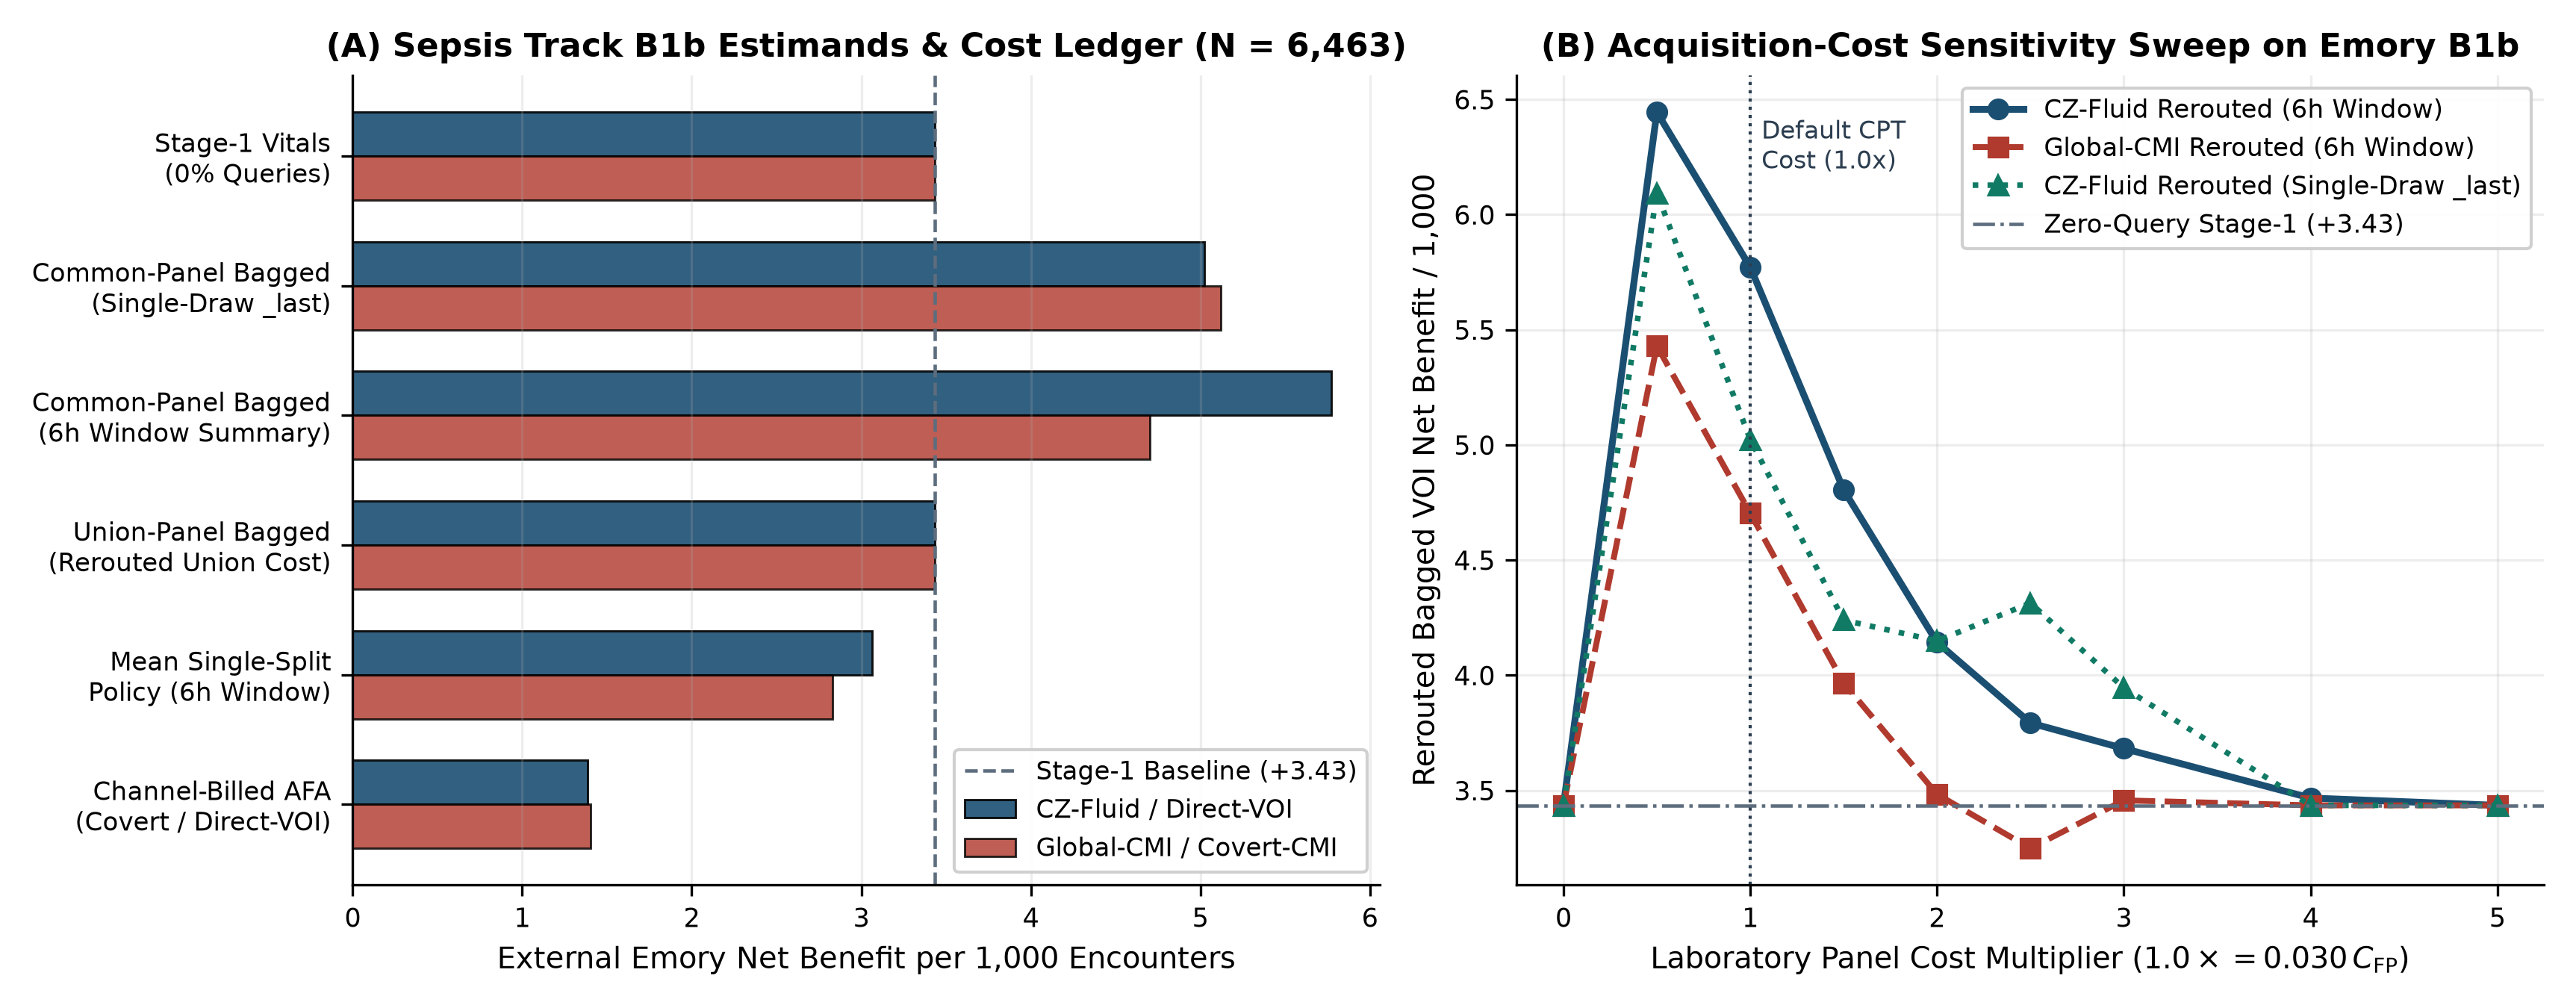
\includegraphics[width=0.98\textwidth]{fig3_sepsis_ledger_and_factorial.png}
\caption{External Emory sepsis utility across deployment estimands and acquisition-cost multipliers ($N=6{,}463$). \textbf{(A)} Comparison of Common-Panel Bagged VOI (single-draw \texttt{\_last} vs.\ $6\text{h}$ window summaries), rerouted Union-Panel Bagged VOI, Mean Single-Split Policy, and patient-level Channel-Billed AFA. \textbf{(B)} Cost-rerouted Net Benefit across panel-cost multipliers $0.0\times\text{--}5.0\times$.}
\label{fig:fig3}
\end{figure}

\subsection{Observation-Horizon Geometry, Prior-Shift Taxonomy, and Assay Availability}
\label{sec:res_horizons}

Figure~\ref{fig:fig4} and Table~\ref{tab:horizons_shift} resolve three critical clinical interpretation questions:
\begin{enumerate}
  \item \textbf{Retiring the $6\text{h}$ Mechanistic Interpretation via $2\text{D}$ Landmark $\times$ Horizon Analysis:} Evaluating $4\text{h}, 6\text{h}, 8\text{h},$ and $12\text{h}$ ICU observation windows against fixed future prediction horizons ($\text{next }2\text{h}, 6\text{h}, 12\text{h}$, and $\text{remaining stay}$) demonstrates that ICU observation time does \emph{not} equate to PhysioNet's $6\text{h}$ pre-onset Sepsis-3 label window. At the $6\text{h}$ landmark ($349$ remaining-stay Emory events), only $16$ ($4.6\%, \pi=0.25\%$), $36$ ($10.3\%, \pi=0.56\%$), and $78$ ($22.3\%, \pi=1.21\%$) events occur within the next $2\text{h}$, $6\text{h}$, and $12\text{h}$, whereas $\mathbf{271/349}$ ($\mathbf{77.7\%}$) occur $>12\text{h}$ later in the stay (Figure~\ref{fig:fig4}A). At short fixed horizons ($\pi \le 1.21\% \ll \tau^*=6.25\%$), VOI routing abstains ($\Delta\text{NB}=0.00\text{--}0.03$), showing that $6\text{h}$ remaining-stay performance reflects cohort composition and cumulative stay prevalence rather than an acute $6\text{h}$ pre-onset physiological boundary. Removing all direct SOFA organ-score channels (\texttt{Creatinine/BUN, Bilirubin, Platelets, Blood Gas}) leaves \texttt{Lactate\_last} selection and utility completely unchanged ($+5.02 / +5.12$), whereas additionally removing \texttt{Lactate} yields zero selected channels ($+3.43$).
  \item \textbf{Unlabeled EM Failure vs.\ Historical Prior-Shift Adaptation:} On Track B2 ($4\text{h}+2\text{h}$ gap; $\pi_{\text{src}}=6.94\% \to \pi_{\text{tgt}}=4.14\%$), zero-shot transfer yields $\operatorname{NB}=-2.55$ ($\texttt{CITL}=-0.385, \texttt{ICI}=0.0208$) on a $75\%$ Emory evaluation holdout ($N=14{,}755$). Purely unlabeled \citet{saerens2002adjusting} EM mixture estimation collapses to the boundary ($\hat{\pi}_{\text{EM}}=10^{-5}, \operatorname{NB}=0.00$) under modest bedside discrimination ($\text{AUROC}\approx 0.60$) and cross-hospital covariate shift (and likewise misestimates prevalence on shifted Yale campuses). Conversely, estimating historical target prevalence on a disjoint $25\%$ Emory slice ($\hat{\pi}_{\text{hist}}=3.99\%, \Delta_0=-0.59$) cuts holdout $\texttt{ICI}$ from $0.0208$ to $\mathbf{0.0082}$ and restores positive utility ($\mathbf{+2.36}/1{,}000$), matching the oracle target-prevalence upper bound ($+2.00/1{,}000$) and remaining positive across $\pm 1.5\text{ pp}$ prevalence estimation error (Figure~\ref{fig:fig4}B).
  \item \textbf{Clinician-Ordering Confounding and Observational Positivity:} Even inside the measured \texttt{Creatinine + WBC} Track B1b cohort, only core admission chemistries/CBC are near-universally observed ($99.4\%\text{--}100\%$), whereas \texttt{Lactate} is physically measured in $32.2\%$ of BIDMC ($50.1\%$ if $Y=1$ vs.\ $30.6\%$ if $Y=0$) and $17.0\%$ of Emory ($35.2\%$ vs.\ $16.0\%$), \texttt{Blood Gas} in $99.7\%$ vs.\ $21.3\%$, and \texttt{Troponin-I} in $1.6\%$ vs.\ $34.6\%$ (Appendix Table~\ref{tab:missingness_avail}). Calibration varies sharply across measurement-intensity strata ($\texttt{ICI}=0.0355$ for $6\text{--}8$ drawn channels vs.\ $0.0083$ for $9\text{--}14$), underscoring that observational acquisition evaluates available EHR states rather than unconfounded prospective testing \citep{vonkleist2025evaluation}.
\end{enumerate}

\begin{table}[t!]
\centering
\caption{Event-time horizon matrix ($W \in \{4,6,8,12\}\text{h} \times$ fixed vs.\ remaining-stay horizons on Emory measured bloodwork) and Track B2 prior-shift adaptation taxonomy ($75\%$ untouched Emory holdout, $N=14{,}755$).}
\label{tab:horizons_shift}
\small
\resizebox{\textwidth}{!}{%
\begin{tabular}{llccccc}
\toprule
\textbf{Analysis} & \textbf{Condition / Adaptation Method} & \textbf{Uses Target $Y$?} & \textbf{Emory Events ($\pi\%$)} & \textbf{Calibration (\texttt{CITL} \,|\, \texttt{ICI})} & \textbf{Glob / CZ NB $/1\text{k}$} & \textbf{Contrast / Finding} \\
\midrule
\multirow{4}{*}{\shortstack[l]{\textbf{$2\text{D}$ Horizon Audit}\\(at $W=6\text{h}, N=6{,}463$;\\$R=6$ compact splits)}}
  & Predict Next $2\text{h}$ & Eval.\ only & $16$ ($0.25\%$) & --- & $0.00 / 0.00$ & $\pi \ll \tau^*$: $0\%$ queries \\
  & Predict Next $6\text{h}$ & Eval.\ only & $36$ ($0.56\%$) & --- & $0.00 / 0.00$ & Only $10.3\%$ of stay events \\
  & Predict Next $12\text{h}$ & Eval.\ only & $78$ ($1.21\%$) & --- & $+0.26 / +0.29$ & $+0.03$ ($[0.00,+0.06], 0.0004$) \\
  & Predict Remaining ICU Stay & Eval.\ only & $349$ ($5.40\%$) & --- & $+3.19 / \mathbf{+5.04}$ & $77.7\%$ occur $>12\text{h}$ post-$6\text{h}$ \\
\midrule
\multirow{4}{*}{\shortstack[l]{\textbf{Track B2 Prior Shift}\\($6.94\% \to 4.20\%$ on\\$75\%$ Emory holdout)}}
  & Zero-Shot Unadjusted ($\hat{\pi}=6.94\%$) & None & $619$ ($4.20\%$) & $-0.385$ \,|\, $0.0208$ & --- / $-2.55$ & Severe risk overprediction \\
  & Unlabeled \citet{saerens2002adjusting} EM & None ($0$ labels) & $619$ ($4.20\%$) & $+8.533$ \,|\, $0.0423$ & --- / $0.00$ & Boundary collapse ($\hat{\pi}=10^{-5}$) \\
  & \textbf{Disjoint $25\%$ Historical Prior ($\hat{\pi}=3.99\%$)} & Separate $25\%$ slice & $619$ ($4.20\%$) & $+0.202$ \,|\, $\mathbf{0.0082}$ & --- / $\mathbf{+2.36}$ & Restores utility ($\Delta_0=-0.59$) \\
  & Oracle Holdout Prevalence ($\pi=4.20\%$) & Aggregate oracle & $619$ ($4.20\%$) & $+0.149$ \,|\, $\mathbf{0.0072}$ & --- / $+2.00$ & Theoretical prior-shift bound \\
\bottomrule
\end{tabular}%
}
\end{table}

\begin{figure}[t!]
\centering
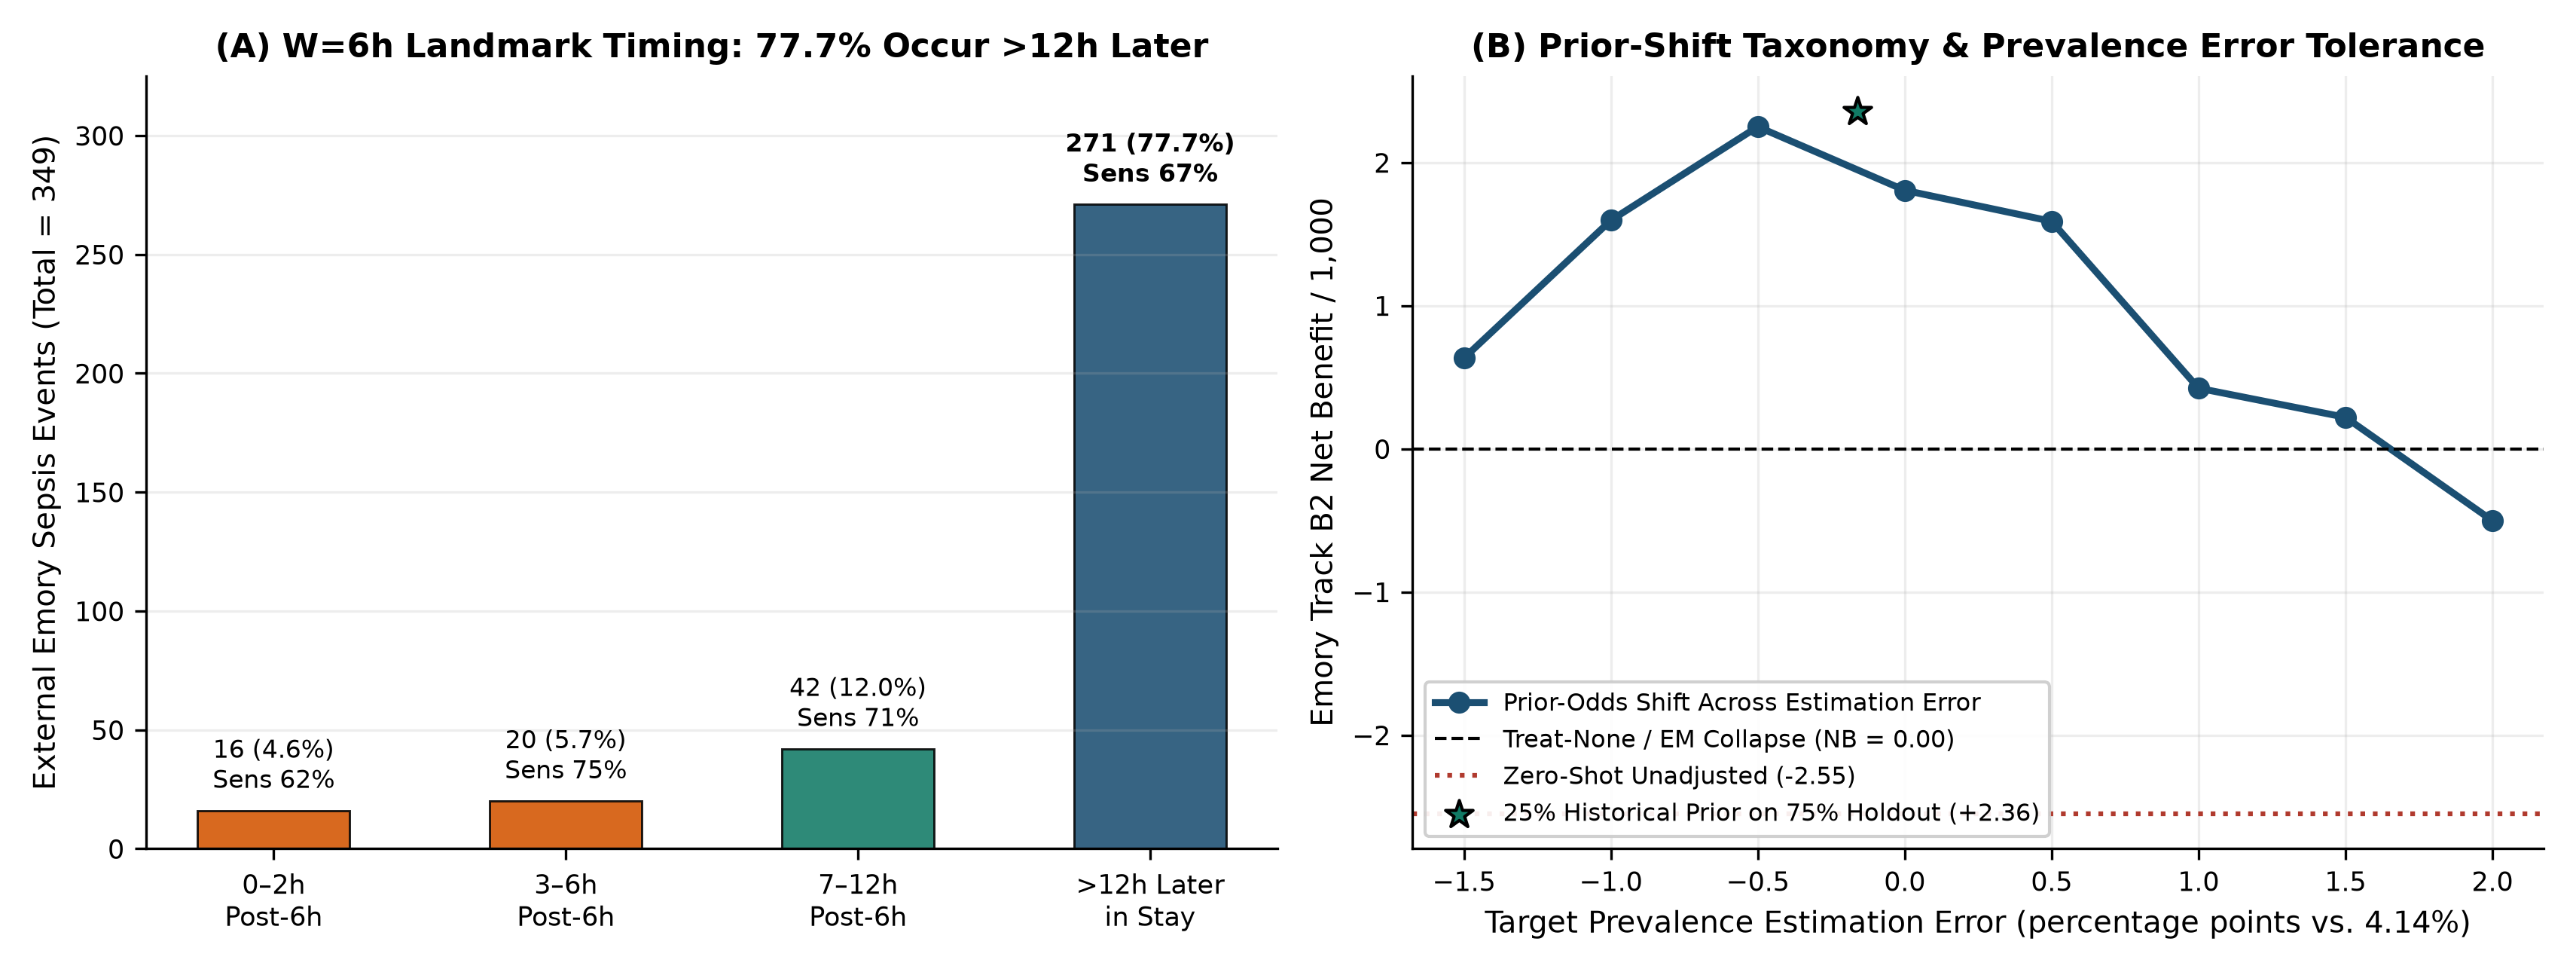
\includegraphics[width=0.98\textwidth]{fig4_horizons_shift_and_missingness.png}
\caption{Event-time horizon distribution and prior-shift tolerance. \textbf{(A)} Distribution of actual lead times from the $6\text{h}$ ICU landmark to \texttt{SepsisLabel} positivity across $349$ Emory cases, showing $77.7\%$ occur $>12\text{h}$ later. \textbf{(B)} Track B2 Net Benefit across target-prevalence estimation errors ($-1.5$ to $+2.0\text{ pp}$), contrasting zero-shot transfer, unlabeled EM collapse, and disjoint $25\%$ historical prior adaptation.}
\label{fig:fig4}
\end{figure}

\subsection{Multi-Campus Yale ED Transfer Including Untested Campus C and Governance Audits}
\label{sec:res_yale}

Table~\ref{tab:yale_results} and Figure~\ref{fig:fig5} report Common-Panel Bagged VOI across all Yale ED cross-campus transfers (Campus A $\to$ Campus B and previously untested Campus C) and within-system reference benchmarks:
\begin{itemize}
  \item \textbf{Low-Acuity \texttt{ESI 4--5} Cross-Campus Transfer (Campus B \& Untested Campus C):} On Campus A ($70{,}360$ visits), \texttt{Global-CMI} locks three HIE/medication modules ($C=0.030$), whereas \texttt{CZ-Beta} halts after two medication modules ($C=0.021$) and damps $\hat{\beta}_{\text{CZ}}=0.17$. On Campus B ($N=51{,}205$), \texttt{CZ-Fluid} ties \texttt{Global-CMI} ($+5.22$ vs.\ $+5.20/1{,}000$; $\Delta\text{NB}=+0.03$, $95\%$ CI $[-0.25, +0.31]$, $p_{\text{DH}}=0.828$; $+\mathbf{1.59}$ over Triage, $p_{\text{DH}}=0.0002$). On previously untested \textbf{Campus C} ($N=31{,}430, 616$ admissions, $\pi=1.96\%$), avoiding the third module fee yields $\mathbf{+5.20}$ versus $+4.70/1{,}000$ ($\mathbf{\Delta\text{NB}=+0.50}$, $95\%$ CI $[+0.19, +0.82]$, $p_{\text{DH}}=\mathbf{0.0022}$, exceeding the $0.25/1{,}000$ \texttt{MCID} in point estimate; $+\mathbf{2.73}$ over Triage, $p_{\text{DH}}=0.0002$). Within-system blinded OOF reference Track B3 ($N=152{,}995$) remains $-0.12/1{,}000$ ($[-0.24, -0.0001], p_{\text{DH}}=0.050$, inside $\pm 0.25$ \texttt{MCID}).
  \item \textbf{All-Comers Cross-Campus Transfer (Campus B \& Untested Campus C):} Both methods lock the identical three-module panel ($C=0.024$), isolating KL-gated Stage-2 specialization ($\hat{\beta}_{\text{CZ}}=0.49$). \texttt{CZ-Fluid} improves Common-Panel Bagged NB on Campus B ($N=166{,}497, \pi=31.65\%$) by $\mathbf{+0.39}/1{,}000$ ($273.29$ vs.\ $272.91$, $95\%$ CI $[+0.22, +0.55]$, $p_{\text{DH}}=0.0002$) and on community \textbf{Campus C} ($N=71{,}706, \pi=15.62\%$) by $\mathbf{+0.23}/1{,}000$ ($108.77$ vs.\ $108.53$, $95\%$ CI $[+0.01, +0.47]$, $p_{\text{DH}}=0.0412$; $+5.08$ over Triage), though both point estimates lie near or below the $0.40/1{,}000$ all-comer \texttt{MCID}.
  \item \textbf{Subgroup Utility and Repeated-Sampling Conformal Governance (Figure~\ref{fig:fig5}B, Appendix~\ref{app:clinical_gov}):} Across $10$ external Campus B+C \texttt{ESI 4--5} demographic/payer strata (Appendix Table~\ref{tab:fairness}), \texttt{CZ-Fluid} improves over Triage in $9/10$ groups (remaining negative at $-1.27$ vs.\ $-1.36$ Global-CMI in low-prevalence \texttt{Other/Self-Pay}, $\pi=0.82\%, \texttt{CITL}=-1.07$) and exceeds \texttt{Global-CMI} nominally in non-English ($+0.70, p_{\text{DH}}=0.002$) and \texttt{race:Other} ($+0.67, p_{\text{DH}}=0.018$) visits while matching across remaining strata. For Conformal Benjamini--Hochberg (\texttt{CfBH}) alerting at $\alpha_{\text{FDR}}=0.75$ ($\text{PPV}\ge 25\%$), zero-shot Campus A calibration inflates Campus B alerts to $90.0/100$ visits ($\text{FDP}=98.0\%$). Across $R=200$ disjoint local burn-in splits (Figure~\ref{fig:fig5}B, Appendix Table~\ref{tab:cfbh_burnin}), any $n_{\text{burn}} \ge 250$ controls marginal $\text{FDR} = \mathbb{E}[\text{FDP}] \le 0.75$ ($63.4\%\text{--}70.9\%$), reducing alerts to $6.2/100$ ($30.8\%$ recall at $n_{\text{burn}}=250$) and $2.2/100$ ($15.9\%$ recall at $n_{\text{burn}}=2{,}000$), though single-split realized FDP remains bimodal ($95\%$ interval $[0.00, 0.89]$) at $1.81\%$ admission prevalence.
\end{itemize}

\begin{table}[t!]
\centering
\caption{Yale New Haven Health System cross-campus Common-Panel Bagged VOI evaluations (Campus A $\to$ Campus B and previously untested Campus C; $B=10{,}000$ paired bootstraps) and within-system reference benchmarks.}
\label{tab:yale_results}
\small
\resizebox{\textwidth}{!}{%
\begin{tabular}{llcccccc}
\toprule
\textbf{Yale Evaluation Cohort} & \textbf{$N_{\text{ext}}$ ($\pi\%$)} & \textbf{Stage-1 NB} & \textbf{Global-CMI NB ($q\%$)} & \textbf{CZ-Fluid NB ($q\%$)} & \textbf{CZ vs.\ Global-CMI ($95\%$ CI, $p_{\text{DH}}$)} & \textbf{CZ vs.\ Stage-1} & \textbf{CZ \texttt{CITL} \,|\, \texttt{ICI}} \\
\midrule
\textbf{Campus A $\to$ B:} ESI 4--5 & $51{,}205$ ($1.81\%$) & $+3.63$ & $+5.20$ ($67.3\%$) & $\mathbf{+5.22}$ ($70.1\%$) & $+0.03$ ($[-0.25,+0.31], 0.828$) & $\mathbf{+1.59}$ ($0.0002$) & $-0.82$ \,|\, $0.0167$ \\
\textbf{Campus A $\to$ C (Untested):} ESI 4--5 & $31{,}430$ ($1.96\%$) & $+2.47$ & $+4.70$ ($72.9\%$) & $\mathbf{+5.20}$ ($74.8\%$) & $\mathbf{+0.50}$ ($\mathbf{[+0.19,+0.82], 0.0022}$) & $\mathbf{+2.73}$ ($0.0002$) & $-0.66$ \,|\, $0.0144$ \\
\textbf{Campus A $\to$ B:} All-Comers & $166{,}497$ ($31.65\%$) & $271.06$ & $272.91$ ($33.3\%$) & $\mathbf{273.29}$ ($32.4\%$) & $\mathbf{+0.39}$ ($\mathbf{[+0.22,+0.55], 0.0002}$) & $\mathbf{+2.24}$ ($0.0002$) & $+0.08$ \,|\, $0.0126$ \\
\textbf{Campus A $\to$ C (Untested):} All-Comers & $71{,}706$ ($15.62\%$) & $103.68$ & $108.53$ ($43.4\%$) & $\mathbf{108.77}$ ($42.4\%$) & $\mathbf{+0.23}$ ($\mathbf{[+0.01,+0.47], 0.0412}$) & $\mathbf{+5.08}$ ($0.0002$) & $-0.51$ \,|\, $0.0511$ \\
\midrule
\textbf{Ref.\ Within-System B3:} Blinded ESI 4--5 & $152{,}995$ ($1.88\%$) & $+4.63$ & $\mathbf{+7.25}$ (OOF) & $+7.13$ (OOF) & $-0.12$ ($[-0.24,-0.0001], 0.050$) & $+2.50$ ($0.0002$) & $-0.002$ \,|\, $0.0014$ \\
\bottomrule
\end{tabular}%
}
\end{table}

\begin{figure}[t!]
\centering
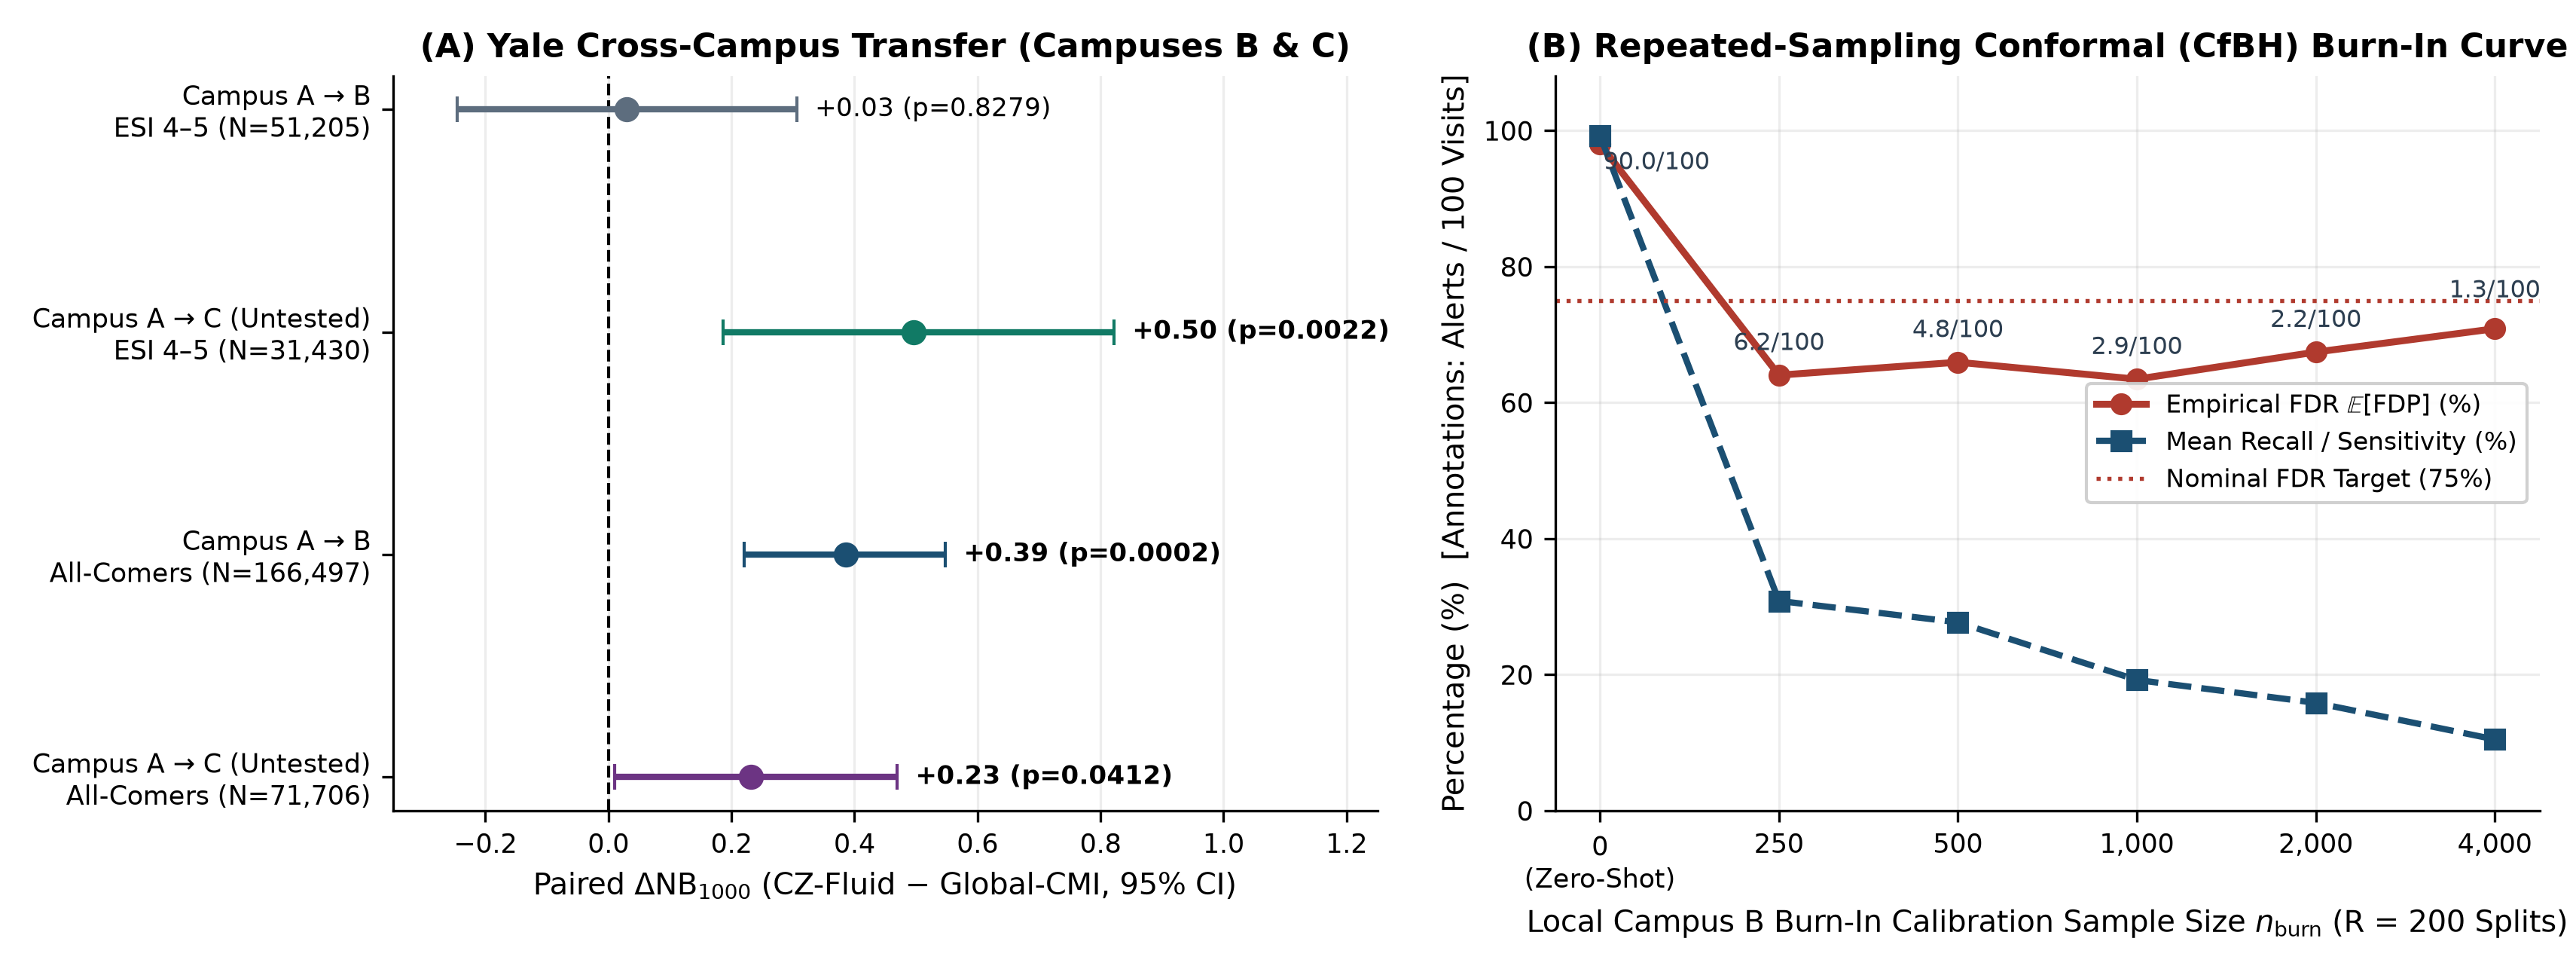
\includegraphics[width=0.98\textwidth]{fig5_yale_campuses_and_cfbh_governance.png}
\caption{Yale ED cross-campus transfer and repeated-sampling conformal governance. \textbf{(A)} Paired $\Delta\operatorname{NB}_{1000}$ (\texttt{CZ-Fluid} minus \texttt{Global-CMI}, $95\%$ CIs) under Common-Panel Bagged VOI across Campus B and previously untested Campus C. \textbf{(B)} Empirical $\text{FDR}=\mathbb{E}[\text{FDP}]$, mean recall, and alerts per $100$ visits across $R=200$ disjoint Campus B conformal burn-in splits.}
\label{fig:fig5}
\end{figure}

\section{Discussion, Practical Guidance, and Limitations}
\label{sec:discussion}

Our theoretical corrections, factorial experiments, and panel-costed clinical benchmarks refine when threshold-aware feature acquisition should---and should not---replace conventional global pipelines:
\begin{enumerate}
  \item \textbf{When Threshold-Aware Acquisition Wins vs.\ When Global Learning Suffices:} Both the $36$-cell synthetic regime map and the clinical cohorts tell a consistent story. When a single dominant Stage-2 predictor acts monotonically across risk strata without competing subthreshold decoys (e.g., single-draw \texttt{Lactate\_last} on Track B1b, or outpatient medication counts on Campus B \texttt{ESI 4--5}), global log-loss discovery and standard Stage-2 learners already capture the decision-relevant signal ($+5.12$ vs.\ $+5.02$; $+5.20$ vs.\ $+5.22$). Conversely, when subthreshold features compete for finite discovery budgets (Campus C \texttt{ESI 4--5}, where \texttt{CZ-Beta} avoids an uninformative third module fee for $+0.50/1{,}000$; synthetic decoy competition in $23/24$ regime cells) or multi-feature trajectory summaries interact near $\tau^*$ ($6\text{h}$ sepsis window $+5.77$ vs.\ $+4.70$, and $166\text{k}/71\text{k}$ ED all-comers), coordinating discovery and residual specialization via Beta--KL threshold geometry yields consistent gains while smooth properness avoids the finite-pilot variance of direct step-function utility optimization.
  \item \textbf{Cost Accounting Must Match Physical Acquisition Workflows:} Replacing flat binary query billing with explicit procedure-plus-assay ledgers demonstrates that ensemble predictions are deployable only when all ensemble members share a locked panel $\mathcal{S}_{\text{common}}$ (or price the full union of required channels), and that Stage-A discovery should normalize gains by total incremental procedure-plus-assay cost when procedures differ (e.g., arterial puncture vs.\ routine venipuncture).
  \item \textbf{Limitations:} First, all clinical evaluations are retrospective observational benchmarks subject to clinician-ordering selection and incomplete counterfactual assay availability (\citealp{agniel2018biases,vonkleist2025evaluation}; \texttt{Lactate} physically drawn in $17.0\%$ of Emory Track B1b). Second, primary Emory sepsis event counts ($349$ events) yield wide uncertainty intervals: on $6\text{h}$ summaries, \texttt{CZ-Fluid}'s $+1.07/1{,}000$ gain over \texttt{Global-CMI} is not statistically significant at $\alpha=0.05$ ($p_{\text{DH}}=0.094$), and single-pilot hyperparameter sweeps exhibit discrete Holm-boundary sensitivity across $9$ $(\kappa_{\max}, B_{\text{score}})$ configurations (Appendix Table~\ref{tab:sens_9grid}). Third, in \citet{hong2018predicting}'s public ED dataset, repeat-visit patient linkage is unavailable (\texttt{pat\_mrn\_id} is encounter-level), and Campus C previously appeared in pooled within-system reference runs prior to its first cross-campus evaluation here. Fourth, unlabeled EM prior-shift estimation fails under joint covariate and prevalence shift, requiring historical or local burn-in target data before deployment.
\end{enumerate}

\section*{Author Contributions, Funding, and Conflicts of Interest}

Conceptualization, methodology, software, validation, formal analysis, investigation, data curation, and writing: W.A.S. This research received no external grant funding. The author declares no conflicts of interest.

\section*{Institutional Review Board and Informed Consent Statement}

Conducted in accordance with the Declaration of Helsinki and $45\text{ CFR }46.102\text{(e)}$ using publicly available, IRB-approved, de-identified \texttt{CC BY 4.0} benchmark datasets: PhysioNet/CinC Challenge 2019 \citep{goldberger2000physionet,reyna2020early} (BIDMC and Emory IRB waivers) and Yale New Haven Health System ED Triage \citep{hong2018predicting} (Yale HIC \texttt{IRB \#2000021295}). No human participants were recruited and no clinical interventions were performed; retrospective methodological benchmarks are not cleared for clinical care without prospective validation and local governance.

\section*{Data and Code Availability Statement}

{\raggedright The \texttt{collision-zone-ed} package (MIT License; Release \texttt{v2.3.0}, code commit \texttt{5362988}; preprint archived on \texttt{Preprints.org}), \texttt{PanelCostSchedule} ledger, factorial and horizon runners (\texttt{scripts/run\_paper2\_v2\_3\_remediation.py}), deterministic $<1\text{s}$ checkpoint-to-table verifier (\texttt{scripts/verify\_paper2\_v3\_tables.py}), modular JSON checkpoints (\texttt{results/v2\_3\_blocks/}), pinned environment (\texttt{requirements-lock.txt}), RNG seed manifest (\texttt{SEED\_MANIFEST.md}), and $50/50$ passing \texttt{pytest} suite are openly available at \url{https://github.com/deesatzed/collision-zone-ed} (documentation: \url{https://deesatzed.github.io/collision-zone-ed/}). Clinical datasets are available via PhysioNet (\url{https://physionet.org/content/challenge-2019/1.0.0/}) and Yale ED (\url{https://github.com/yaleemmlc/admissionprediction}).\par}

\section*{AI-Assisted Workflows Disclosure and Acknowledgments}

In accordance with COPE transparency standards, portions of the computational workflow---bibliographic cross-checking, Python pipeline implementation, numerical formula verification, and manuscript drafting---were conducted using \emph{Google Antigravity} powered by \emph{Gemini Pro} models (no external scientific database connectors were used, and no generative AI generated or altered primary empirical data). All design decisions, mathematical proofs, code executions, citations, and text were independently verified and approved by the human author. Computational research access was provided through the \emph{Google Antigravity for Science} program; we thank the maintainers of \texttt{PhysioNet} \citep{goldberger2000physionet}, \citet{reyna2020early}, \citet{hong2018predicting}, \texttt{LightGBM} \citep{ke2017lightgbm}, \texttt{SciPy} \citep{virtanen2020scipy}, and \texttt{scikit-learn} \citep{pedregosa2011scikit}.

\appendix

\section{Mathematical Derivations, Proofs, and Scope Qualifications}
\label{app:proofs}

\begin{proposition}[Mode-Aligned Beta Proper Score and Exact Boltzmann KL Identity; \citealp{schervish1989general,buja2005loss}]
\label{prop:unification}
For $\tau^* \in (0,1)$ and $\kappa > 0$, let $\alpha = 1 + \kappa\tau^*$, $\beta = 1 + \kappa(1-\tau^*)$, and $w_{\tau^*,\kappa}(\tau) = \tau^{\alpha-1}(1-\tau)^{\beta-1}/B(\alpha,\beta)$.
\begin{enumerate}
  \item Substituting $w_{\tau^*,\kappa}$ into Schervish's integral representation $S_w(y,p) = -y\int_p^1(1-\tau)w(\tau)\,d\tau - (1-y)\int_0^p \tau w(\tau)\,d\tau$ yields the strictly proper closed-form score
  \begin{equation}
    S_{\tau^*,\kappa}(y, p) = -y\,\frac{\beta}{\alpha+\beta}\big(1 - I_p(\alpha, \beta+1)\big) - (1-y)\,\frac{\alpha}{\alpha+\beta}\, I_p(\alpha+1, \beta),
    \label{eq:schervish_closed}
  \end{equation}
  where $I_p(a,b)$ is the regularized incomplete beta function \citep{buja2005loss,gneiting2007strictly}.
  \item Dividing $w_{\tau^*,\kappa}(p)$ by its unique maximum $w_{\tau^*,\kappa}(\tau^*) = (\tau^*)^{\kappa\tau^*}(1-\tau^*)^{\kappa(1-\tau^*)}/B(\alpha,\beta)$ yields
  \[
    \log\!\left[\frac{w_{\tau^*,\kappa}(p)}{w_{\tau^*,\kappa}(\tau^*)}\right] = -\kappa\left[\tau^*\log\frac{\tau^*}{p} + (1-\tau^*)\log\frac{1-\tau^*}{1-p}\right] = -\kappa\, D_{\text{KL}}\!\big(\operatorname{Bern}(\tau^*)\,\|\,\operatorname{Bern}(p)\big),
  \]
  establishing Eq.~\eqref{eq:beta_kl_identity} identically.
  \item For small additive probability perturbations $\delta \to 0$ at $p \ll \tau^*$, local Bregman divergence scales as $\tfrac{1}{2}w_{\tau^*,\kappa}(p)\delta^2 = \Theta(p^{\kappa\tau^*}\delta^2)$ versus $\Theta(p^{-1}\delta^2)$ under log-loss (noting that proportional updates $\delta \propto p$ yield $O(p) \to 0$ under log-loss and $O(p^{2+\kappa\tau^*}) \to 0$ under $S_{\tau^*,\kappa}$).
\end{enumerate}
\end{proposition}

\textbf{Finite-Capacity Counterexample to Population Conditional-Independence Null Non-Positivity:} Let $X_1, X_2 \stackrel{\text{i.i.d.}}{\sim} \operatorname{Bern}(0.5)$, $Y = X_1 \oplus X_2$, and $Z = X_1 \oplus X_2$. Although $I(Y; Z \mid X_1, X_2) = 0$ identically, depth-$1$ axis-aligned decision stumps on $(X_1, X_2)$ achieve only chance risk ($\mathbb{E}[\ell] = -\log 2$), whereas depth-$1$ stumps on $(X_1, X_2, Z)$ achieve zero risk, yielding positive expected out-of-fold gain ($\Delta \hat{S} > 0.30$ verified in \texttt{test\_three\_predicates\_v3.py}). Consequently, Stage-A inference addresses the \emph{learner-specific predictive-utility null}:

\begin{assumption}[Learner-Specific Predictive-Utility Null]
\label{assump:null_nonpos}
At step $t$ with selected set $\mathcal{S}_{t-1}$, channel $m \notin \mathcal{S}_{t-1}$ belongs to the learner-specific predictive-utility null $\mathcal{H}_0^{\mathcal{A}}(\mathcal{S}_{t-1})$ if augmenting learner $\mathcal{A}$ with $Z_m$ does not improve expected out-of-sample $S_{\tau^*,\kappa}$ score: $\mu_{m,N} \equiv \mathbb{E}[N^{-1}\sum_{i=1}^N \psi_{i,m\mid\mathcal{S}_{t-1}}] \le 0$.
\end{assumption}

\begin{theorem}[Two-Phase Variance SRS Reduction and Conditional Split-Pilot Inference]
\label{thm:hsfp_neyman}
Let $\mathcal{P} = \mathcal{P}_{\text{fit}} \sqcup \mathcal{P}_{\text{conf}}$ be a stratified without-replacement Phase-2 pilot split within each stratum $h \in \{1,\dots,H\}$ so candidate predictors are fit strictly on $\mathcal{P}_{\text{fit}}$ and evaluated on $\mathcal{P}_{\text{conf}}$ ($n_{\text{conf}} = |\mathcal{P}_{\text{conf}}|$, stratum sizes $n_{h,\text{conf}} \ge 2$, HT weights $w_i = N_h / n_{h,\text{conf}}$, residuals $r_i = \psi_i - \hat{G}$).
\begin{enumerate}
  \item Conditional on $(\mathcal{D}_{\text{train}}, \mathcal{P}_{\text{fit}})$, the scores $\{\psi_i\}_{i \notin \mathcal{P}_{\text{fit}}}$ are fixed finite-population quantities, so $\hat{G} = N^{-1}\sum_{i\in\mathcal{P}_{\text{conf}}} w_i \psi_i$ is design-unbiased for the remaining-frame mean and the implemented two-phase variance estimator
  \begin{equation}
    \widehat{V}_{\text{total}} = \underbrace{\frac{n_{\text{conf}}}{n_{\text{conf}}-1}\frac{1}{N^2}\sum_{i \in \mathcal{P}_{\text{conf}}} w_i r_i^2}_{\widehat{V}_{\text{I}}} + \underbrace{\frac{1}{N^2}\sum_{h=1}^H N_h^2 \left(1 - \frac{n_{h,\text{conf}}}{N_h}\right)\frac{s_h^2}{n_{h,\text{conf}}}}_{\widehat{V}_{\text{II}}}
    \label{eq:two_phase_var}
  \end{equation}
  reduces identically to $s^2 / n_{\text{conf}}$ under simple random sampling ($H=1, w_i = N/n_{\text{conf}}, \sum r_i^2 = (n_{\text{conf}}-1)s^2 \implies \widehat{V}_{\text{I}} = s^2/N$ and $\widehat{V}_{\text{II}} = (1 - n_{\text{conf}}/N)s^2/n_{\text{conf}}$, summing to $s^2/n_{\text{conf}}$).
  \item Under Assumption~\ref{assump:null_nonpos}, asymptotic normality of studentized HT gains \citep{williamson2021nonparametric}, and consistent ordering of non-null channels ahead of $\mathcal{H}_0^{\mathcal{A}}$ (or at step $t=1$ for a fixed candidate family), Holm step-down rejection at level $\alpha$ controls asymptotic FWER $\le \alpha$. When $4$-fold cross-fitting on full $\mathcal{P}$ replaces sample splitting, $\psi_i$ exhibits weak cross-fold dependence \citep{nadeau2003inference,bates2024crossvalidation}, so Holm stopping serves as an empirically conservative discovery rule rather than an exact finite-sample test.
\end{enumerate}
\end{theorem}

\textbf{Scope of KL-Gated Residual Learning, Martingale VOI, and \texttt{AgnielDeconfounder}:} Under unweighted Bernoulli log-loss $\mathcal{L}(y, f_{\text{glob}}+\pi\Delta_{\text{CZ}})$ with fixed $\pi \in (0,1]$, pointwise differentiation wrt $\Delta_{\text{CZ}}$ gives $g_i = \pi_i(\sigma(f_i)-y_i)$ and $h_i = \pi_i^2\sigma(f_i)(1-\sigma(f_i)) > 0$, so an unconstrained population specialist preserves $\sigma(f^*(x,z))=\mathbb{P}(Y=1\mid X=x,Z=z)$ while L2 leaf penalty $\tilde{\lambda}>0$ shrinks data-starved leaves ($|\hat{\gamma}_\ell^{\text{CZ}}| \le \tilde{\lambda}^{-1}\sum_{i\in R_\ell}\pi_i \to 0$) smoothly to $f_{\text{glob}}(x,z)$; in finite samples, constrained tree depth and regularized OOF stacking approximate this optimum. By concavity of $L^*(p) = C_{\text{FN}}p - (C_{\text{FN}}+C_{\text{FP}})(p-\tau^*)_+$ and $\mathbb{E}[\tilde{P}_2\mid p_1]=p_1$, Jensen's inequality yields Eq.~\eqref{eq:voi_crossing} ($\ge 0$). Finally, if $\tilde{Z} = DZ + (1-D)Z^{\text{imp}}$ matches $P(Z\mid X_{\text{base}}, D=1)$ exactly and $Y \perp Z \mid (X_{\text{base}}, D=1)$, then $\tilde{Z} \perp Y \mid X_{\text{base}}$ despite $Y \not\perp D \mid X_{\text{base}}$; however, linear homoscedastic residual imputation is only a first-moment approximation and cannot identify biological effects among untested patients when ordering depends on unmeasured severity \citep{agniel2018biases,vonkleist2025evaluation}.

\section{Hyperparameter Sensitivity, Missingness Audit, and Governance Tables}
\label{app:sensitivity}
\label{app:horizons_shift}
\label{app:clinical_gov}

Tables~\ref{tab:sens_9grid}--\ref{tab:cfbh_burnin} report the $9$ distinct $(\kappa_{\max}, B_{\text{score}})$ hyperparameter configurations on Emory Track B1b, the $14$-channel physical assay availability audit across BIDMC and Emory, the $10$-subgroup demographic/payer decision-utility audit on pooled external Yale Campuses B and C (\texttt{ESI 4--5}), and the $R=200$ repeated-subsample Campus B \texttt{CfBH} burn-in curves.

\begin{table}[h!]
\centering
\caption{All $9$ distinct $(\kappa_{\max} \in \{12,20,32\} \times B_{\text{score}} \in \{4,8,12\})$ hyperparameter configurations on primary Emory Track B1b Common-Panel Bagged VOI ($N=6{,}463, B=10{,}000$ paired bootstraps; active collision mass on BIDMC exceeds $320$ across all cells, verified to $\max |\Delta \hat{p}_2| \le 6 \times 10^{-8}$ between $M_{\min}=160$ and $320$). Note: here $\kappa_{\max}$ is varied jointly in Stage-A and Stage-2, whereas the primary Table~\ref{tab:sepsis_ledger} specification uses $\kappa_{\text{disc}}=24, \kappa_{\max,\text{S2}}=20$ ($+5.77$ vs.\ $+4.70$, $\Delta=+1.07$).}
\label{tab:sens_9grid}
\footnotesize
\resizebox{\textwidth}{!}{%
\begin{tabular}{ccccccc}
\toprule
\textbf{$B_{\text{score}}$ Bins} & \textbf{$\kappa_{\max}$ (Joint)} & \textbf{$6\text{h}$ CZ / Glob Panel} & \textbf{$6\text{h}$ CZ / Glob Bagged NB} & \textbf{$6\text{h}$ $\Delta$NB ($95\%$ CI, $p_{\text{DH}}$)} & \textbf{\texttt{\_last} CZ / Glob Panel} & \textbf{\texttt{\_last} $\Delta$NB ($p_{\text{DH}}$)} \\
\midrule
$4$ & $12$ & $\emptyset$ / $\emptyset$ & $+3.43 / +3.43$ & $0.00$ ($[0.00, 0.00], 1.00$) & $\emptyset$ / $\emptyset$ & $0.00$ ($1.00$) \\
$4$ & $20$ & $\emptyset$ / $\emptyset$ & $+3.43 / +3.43$ & $0.00$ ($[0.00, 0.00], 1.00$) & $\emptyset$ / $\emptyset$ & $0.00$ ($1.00$) \\
$4$ & $32$ & \texttt{Lactate} / $\emptyset$ & $\mathbf{+5.80} / +3.43$ & $\mathbf{+2.37}$ ($\mathbf{[+0.02, +4.69], 0.0488}$) & \texttt{Lactate} / $\emptyset$ & $+1.64$ ($0.143$) \\
$8$ & $12$ & \texttt{Lactate} / \texttt{Lactate} & $\mathbf{+5.69} / +4.70$ & $+0.99$ ($[-0.28, +2.25], 0.125$) & \texttt{Lactate} / \texttt{Lactate} & $+0.10$ ($0.825$) \\
$8$ & $20$ & $\emptyset$ / \texttt{Lactate} & $+3.43 / +4.70$ & $-1.27$ ($[-3.39, +0.96], 0.253$) & $\emptyset$ / \texttt{Lactate} & $-1.68$ ($0.125$) \\
$8$ & $32$ & \texttt{Lactate} / \texttt{Lactate} & $\mathbf{+5.80} / +4.70$ & $+1.10$ ($[-0.17, +2.36], 0.090$) & \texttt{Glucose} / \texttt{Lactate} & $-2.47$ ($0.019$) \\
$12$ & $12$ & $\emptyset$ / \texttt{BloodGas} & $+3.43 / +4.28$ & $-0.84$ ($[-2.86, +1.31], 0.426$) & $\emptyset$ / \texttt{BloodGas} & $-1.68$ ($0.072$) \\
$12$ & $20$ & $\emptyset$ / \texttt{BloodGas} & $+3.43 / +4.28$ & $-0.84$ ($[-2.86, +1.31], 0.426$) & $\emptyset$ / \texttt{BloodGas} & $-1.68$ ($0.072$) \\
$12$ & $32$ & $\emptyset$ / \texttt{BloodGas} & $+3.43 / +4.28$ & $-0.84$ ($[-2.86, +1.31], 0.426$) & $\emptyset$ / \texttt{BloodGas} & $-1.68$ ($0.072$) \\
\bottomrule
\end{tabular}%
}
\end{table}

\begin{table}[h!]
\centering
\caption{Physical assay availability ($\%$ drawn in hours $1\text{--}6$) across all $14$ candidate CPT channels within Measured-Bloodwork Track B1b (\texttt{Creatinine + WBC} drawn; BIDMC $N=8{,}345$, Emory $N=6{,}463$), stratified by hospital and future sepsis outcome ($Y=0$ vs.\ $Y=1$). In the $1{,}101$ Emory stays ($17.0\%, 123$ events) where \texttt{Lactate} was physically measured, routed AUROC is $0.6272$ (\texttt{CZ-Fluid}) vs.\ $0.6280$ (\texttt{Global-CMI}).}
\label{tab:missingness_avail}
\scriptsize
\resizebox{\textwidth}{!}{%
\begin{tabular}{lcccccc|lcccccc}
\toprule
\textbf{Channel} & \textbf{BIDMC All} & \textbf{$Y=0$} & \textbf{$Y=1$} & \textbf{Emory All} & \textbf{$Y=0$} & \textbf{$Y=1$} & \textbf{Channel} & \textbf{BIDMC All} & \textbf{$Y=0$} & \textbf{$Y=1$} & \textbf{Emory All} & \textbf{$Y=0$} & \textbf{$Y=1$} \\
\midrule
\texttt{lab\_lactate} & $32.2\%$ & $30.6\%$ & $50.1\%$ & $17.0\%$ & $16.0\%$ & $35.2\%$ & \texttt{lab\_glucose} & $99.4\%$ & $99.4\%$ & $99.6\%$ & $100\%$ & $100\%$ & $100\%$ \\
\texttt{lab\_blood\_gas} & $99.7\%$ & $99.7\%$ & $99.7\%$ & $21.3\%$ & $20.1\%$ & $42.7\%$ & \texttt{lab\_ca\_mg\_phos} & $80.0\%$ & $79.0\%$ & $91.6\%$ & $100\%$ & $100\%$ & $100\%$ \\
\texttt{lab\_wbc} & $100\%$ & $100\%$ & $100\%$ & $100\%$ & $100\%$ & $100\%$ & \texttt{lab\_liver\_enz} & $23.5\%$ & $22.7\%$ & $32.2\%$ & $56.5\%$ & $56.0\%$ & $66.8\%$ \\
\texttt{lab\_hemoglobin} & $100\%$ & $100\%$ & $100\%$ & $100\%$ & $100\%$ & $100\%$ & \texttt{lab\_bilirubin} & $22.8\%$ & $22.0\%$ & $30.7\%$ & $56.6\%$ & $56.0\%$ & $67.0\%$ \\
\texttt{lab\_platelets} & $99.5\%$ & $99.5\%$ & $99.4\%$ & $99.9\%$ & $99.9\%$ & $100\%$ & \texttt{lab\_coag\_ptt} & $78.3\%$ & $78.0\%$ & $81.4\%$ & $29.9\%$ & $28.9\%$ & $46.1\%$ \\
\texttt{lab\_renal} & $100\%$ & $100\%$ & $100\%$ & $100\%$ & $100\%$ & $100\%$ & \texttt{lab\_fibrinogen} & $11.7\%$ & $11.4\%$ & $15.3\%$ & $9.4\%$ & $8.8\%$ & $20.1\%$ \\
\texttt{lab\_electrolytes} & $99.8\%$ & $99.9\%$ & $99.6\%$ & $100\%$ & $100\%$ & $100\%$ & \texttt{lab\_troponin\_i} & $1.6\%$ & $1.6\%$ & $1.3\%$ & $34.6\%$ & $34.5\%$ & $37.5\%$ \\
\bottomrule
\end{tabular}%
}
\end{table}

\begin{table}[h!]
\centering
\caption{Subgroup decision utility and calibration audit on pooled external Yale ED Campuses B and C \texttt{ESI 4--5} ($N=82{,}635$; Common-Panel Bagged VOI, $B=5{,}000$ paired bootstraps vs.\ both Stage-1 Triage and \texttt{Global-CMI}).}
\label{tab:fairness}
\scriptsize
\resizebox{\textwidth}{!}{%
\begin{tabular}{lccccccccc}
\toprule
\textbf{Subgroup} & \textbf{$N$ ($\pi\%$)} & \textbf{Query $\%$ (CZ/Glob)} & \textbf{Sens.\ $\%$ (CZ/Glob)} & \textbf{FP $/1\text{k}$ (CZ/Glob)} & \textbf{CZ \texttt{CITL}} & \textbf{NB: Base / Glob / CZ} & \textbf{$\Delta$NB vs.\ Base ($95\%$ CI)} & \textbf{$\Delta$NB vs.\ Glob ($95\%$ CI, $p_{\text{DH}}$)} \\
\midrule
\texttt{lang:English} & $77{,}915$ ($1.88\%$) & $71.8 / 69.2\%$ & $62.9 / 63.1\%$ & $140.0 / 139.5$ & $-0.75$ & $+3.30 / +5.18 / +5.36$ & $+2.06$ ($[+1.54,+2.58]$) & $+0.18$ ($[-0.04,+0.39], 0.108$) \\
\texttt{lang:Non-English} & $4{,}720$ ($1.67\%$) & $74.3 / 72.2\%$ & $51.9 / 49.4\%$ & $124.4 / 125.0$ & $-0.74$ & $+1.43 / +2.15 / +2.85$ & $+1.42$ ($[-0.33,+3.29]$) & $\mathbf{+0.70}$ ($\mathbf{[+0.18,+1.40], 0.0020}$) \\
\midrule
\texttt{race:White} & $39{,}576$ ($2.43\%$) & $73.8 / 72.0\%$ & $68.3 / 68.8\%$ & $179.5 / 178.8$ & $-0.70$ & $+6.02 / +8.33 / +8.45$ & $+2.43$ ($[+1.61,+3.29]$) & $+0.13$ ($[-0.20,+0.46], 0.432$) \\
\texttt{race:Black} & $30{,}102$ ($1.35\%$) & $69.8 / 66.6\%$ & $53.1 / 53.6\%$ & $99.8 / 99.1$ & $-0.82$ & $+0.58 / +2.28 / +2.41$ & $+1.83$ ($[+1.06,+2.58]$) & $+0.13$ ($[-0.16,+0.42], 0.393$) \\
\texttt{race:Other} & $11{,}626$ ($1.32\%$) & $71.2 / 68.1\%$ & $51.0 / 47.7\%$ & $107.9 / 108.1$ & $-0.90$ & $+0.50 / +0.92 / +1.59$ & $+1.09$ ($[-0.06,+2.29]$) & $\mathbf{+0.67}$ ($\mathbf{[+0.12,+1.27], 0.0176}$) \\
\texttt{race:Refused} & $681$ ($1.47\%$) & $69.6 / 66.7\%$ & $70.0 / 70.0\%$ & $105.7 / 104.3$ & $-0.86$ & $+0.98 / +5.10 / +5.27$ & $+4.29$ ($[-0.10,+9.90]$) & $+0.16$ ($[-0.32,+0.64], 0.509$) \\
\midrule
\texttt{ins:Medicaid} & $37{,}132$ ($1.27\%$) & $71.2 / 68.1\%$ & $56.1 / 55.2\%$ & $114.4 / 112.4$ & $-1.04$ & $+0.07 / +1.47 / +1.72$ & $+1.65$ ($[+0.96,+2.31]$) & $+0.25$ ($[-0.03,+0.53], 0.077$) \\
\texttt{ins:Commercial} & $26{,}937$ ($1.91\%$) & $73.5 / 71.1\%$ & $59.6 / 58.8\%$ & $141.2 / 139.5$ & $-0.68$ & $+3.21 / +4.55 / +4.87$ & $+1.66$ ($[+0.68,+2.67]$) & $+0.32$ ($[-0.04,+0.67], 0.076$) \\
\texttt{ins:Medicare} & $10{,}360$ ($4.58\%$) & $73.7 / 73.8\%$ & $76.8 / 78.5\%$ & $261.7 / 272.1$ & $-0.47$ & $+17.35 / +23.65 / +23.59$ & $+6.24$ ($[+4.29,+8.31]$) & $-0.06$ ($[-0.91,+0.72], 0.909$) \\
\texttt{ins:Other/Self} & $8{,}172$ ($0.82\%$) & $67.3 / 64.2\%$ & $37.3 / 37.3\%$ & $89.7 / 86.8$ & $-1.07$ & $-1.15 / -1.36 / -1.27$ & $-0.12$ ($[-1.14,+0.95]$) & $+0.09$ ($[-0.41,+0.60], 0.693$) \\
\bottomrule
\end{tabular}%
}
\end{table}

\begin{table}[h!]
\centering
\caption{Repeated-subsample ($R=200$ disjoint splits per $n_{\text{burn}}$) Campus B \texttt{ESI 4--5} Conformal Benjamini--Hochberg (\texttt{CfBH}) burn-in governance audit ($\alpha_{\text{FDR}}=0.75$, i.e., target $\text{PPV}\ge 25\%$ at $\pi=1.81\%$).}
\label{tab:cfbh_burnin}
\footnotesize
\resizebox{\textwidth}{!}{%
\begin{tabular}{lccccccc}
\toprule
\textbf{Local Burn-In Size $n_{\text{burn}}$} & \textbf{Disjoint Eval.\ $N$} & \textbf{Empirical FDR $\mathbb{E}[\text{FDP}]$} & \textbf{FDP SD ($2.5\%\text{--}97.5\%$ Band)} & \textbf{$\mathbb{P}(\text{FDP} > 0.75)$} & \textbf{Mean Recall $\pm$ SD} & \textbf{TP Yield $/1\text{k}$} & \textbf{Alerts $/100$ Visits} \\
\midrule
$0$ (Zero-Shot Campus A Cal.) & $51{,}205$ & $0.9800$ ($>0.75$) & --- & $1.000$ & $99.24\%$ & $17.97$ & $90.01$ \\
$250$ Campus B Visits & $50{,}955$ & $\mathbf{0.6403}$ ($\le 0.75$) & $0.396$ ($[0.000, 0.954]$) & $0.725$ & $30.83 \pm 25.71\%$ & $5.58$ & $6.21$ \\
$500$ Campus B Visits & $50{,}705$ & $\mathbf{0.6593}$ ($\le 0.75$) & $0.377$ ($[0.000, 0.927]$) & $0.755$ & $27.69 \pm 23.81\%$ & $5.01$ & $4.78$ \\
$1{,}000$ Campus B Visits & $50{,}205$ & $\mathbf{0.6344}$ ($\le 0.75$) & $0.378$ ($[0.000, 0.905]$) & $0.740$ & $19.21 \pm 19.36\%$ & $3.48$ & $2.85$ \\
$2{,}000$ Campus B Visits & $49{,}205$ & $\mathbf{0.6742}$ ($\le 0.75$) & $0.339$ ($[0.000, 0.892]$) & $0.775$ & $15.85 \pm 17.31\%$ & $2.87$ & $2.20$ \\
$4{,}000$ Campus B Visits & $47{,}205$ & $\mathbf{0.7085}$ ($\le 0.75$) & $0.306$ ($[0.000, 0.878]$) & $0.805$ & $10.47 \pm 11.10\%$ & $1.90$ & $1.33$ \\
\bottomrule
\end{tabular}%
}
\end{table}

\clearpage
\section{Version \texttt{v2.3.0} Revision Ledger and TRIPOD+AI Audit}
\label{app:ledger_tripod}

\textbf{Summary of Revisions from Draft \texttt{v2.2} to \texttt{v2.3.0} (Commit \texttt{5362988}):} (1) Replaced flat-$0.03$ heterogeneous-ensemble billing with explicit procedure-plus-assay \texttt{PanelCostSchedule} accounting under Common-Panel Bagged VOI, separating single-draw \texttt{\_last} specimens from $6\text{h}$ retrieval summaries and reporting Union-Panel, Per-Split, Fractionally Billed Ensemble, and Channel-Billed AFA comparators; (2) credited \citet{buja2005loss}, \citet{turney1995cost}, and \citet{bilgic2011value} and unified the architecture via the exact normalized-Beta / Boltzmann-KL identity; (3) corrected printed Eq.~\eqref{eq:two_phase_var} from $w_i^2 r_i^2$ to the implemented $w_i r_i^2$, added the finite-capacity XOR counterexample and disjoint $50/50$ split-pilot confirmation protocol, and distinguished log-loss curvature from local proportional KL gain; (4) added $6\times 2$ synthetic and $5\times 3$ clinical discovery-by-backbone factorials, matched-capacity ungated residual models, scale-invariant $R_{\text{CZ}}$ diagnostics, quadrature Oracle VOI and covariate-enriched VOI audits, and a $36$-cell regime map; and (5) retired the $6\text{h}$ Sepsis-3 mechanistic claim via a $16$-cell landmark-by-horizon matrix, reclassified oracle vs.\ unlabeled EM vs.\ historical prior-shift adaptation, audited $14$-channel availability, evaluated previously untested Yale Campus C ($N=71{,}706$), and replaced single-seed \texttt{CfBH} burn-in with $R=200$ repeated-sampling curves.

% Supplementary Table: 2024 TRIPOD+AI Reporting Audit (Collins et al., BMJ 2024;385:e078378)
\begin{table}[h!]
\centering
\caption{TRIPOD+AI reporting checklist mapping for the retrospective clinical prediction and feature-acquisition evaluations (PhysioNet 2019 ICU Sepsis and Yale New Haven Health System ED Triage; \citealp{collins2024tripodai}).}
\label{tab:tripod_ai}
\scriptsize
\renewcommand{\arraystretch}{1.12}
\begin{tabular}{>{\raggedright\arraybackslash}p{0.12\textwidth}>{\raggedright\arraybackslash}p{0.24\textwidth}>{\raggedright\arraybackslash}p{0.56\textwidth}}
\toprule
\textbf{Section / Item} & \textbf{TRIPOD+AI Requirement} & \textbf{Manuscript Location and Compliance Summary} \\
\midrule
Title (1) & Identify study developing/evaluating a multivariable prediction model using ML & Title specifies threshold-aware feature acquisition and residual learning for clinical prediction; retrospective evaluation explicitly framed in Abstract and Section~\ref{sec:study_design}. \\
Abstract (2) & Structured summary of objectives, data, methods, results, limitations & Narrative $<200$-word Abstract states problem, unified Beta--KL method, synthetic and external hospital cohorts, repaired Common-Panel Bagged VOI results, and retrospective/cost limitations. \\
Background (3a--3b) & Clinical/methodological context, intended role, target threshold & Sections~\ref{sec:intro}--\ref{sec:methods} formulate the Decision-Information Dilution Hypothesis around prespecified clinical threshold $\tau^* = C_{\text{FP}}/(C_{\text{FP}}+C_{\text{FN}})$. \\
Data Sources (4a--4b) & Study design, data sources, dates, eligibility, open-access provenance & Section~\ref{sec:study_design} documents PhysioNet/CinC 2019 ICU cohorts (BIDMC $N=19{,}873$, Emory $N=18{,}359$) and Yale ED cohorts ($N=560{,}486$ across Campuses A, B, and C). \\
Participants (5a--5c) & Setting, inclusion/exclusion criteria, landmark alignment & Causal observation landmarks ($4/6/8/12\text{h}$) exclude pre-landmark \texttt{SepsisLabel}$=1$; measured-bloodwork (Track B1b) vs.\ all-comers (Track A) selection explicitly audited (Appendix~\ref{app:clinical_gov}). \\
Outcome (6a--6c) & Outcome definition, timing/horizon, incorporation-bias assessment & Section~\ref{sec:res_sepsis} and Appendix~\ref{app:horizons_shift} separate ICU observation window from fixed future prediction horizons ($2\text{h}, 6\text{h}, 12\text{h}$, remaining stay) and audit SOFA-constituent incorporation bias. \\
Predictors (7a--7c) & Baseline vs.\ Stage-2 channels, point-in-time availability, cost ledger & Section~\ref{sec:methods} distinguishes bedside Stage-1 predictors from Stage-2 laboratory panels (single-draw \texttt{\_last} vs.\ $6\text{h}$ retrieval summaries) and prices procedure + CPT assay costs via \texttt{PanelCostSchedule}. \\
Sample Size (8) & Cohort sizes, event counts, finite-sample power constraints & Exact $N$ and event counts reported in every table ($349$ external events in Emory Track B1b; $616$ events in Yale Campus C ESI 4--5); split-pilot power loss quantified in Appendix~\ref{app:proofs}. \\
Missing Data (9) & Missingness rates by site/outcome, handling, ordering confounding & Appendix Table~\ref{tab:missingness_avail} reports per-channel availability across sites and outcomes ($Y=0$ vs.\ $Y=1$), complete-panel subset results, and \texttt{AgnielDeconfounder} / \citet{vonkleist2025evaluation} observability assumptions. \\
Analytical Methods (10a--10f) & Learner architectures, hyperparameter tuning, OOF stacking, VOI routing & Section~\ref{sec:methods} and Appendix~\ref{app:proofs} specify LightGBM capacities, 3-fold OOF stacking, empirical martingale VOI offset, and disjoint $\mathcal{D}_{\text{train}}/\mathcal{D}_{\text{cal}}/\mathcal{D}_{\text{test}}$ splits. \\
Fairness / Subgroups (11) & Treatment of sociodemographic attributes and subgroup evaluation & Nine demographic/payer/site variables stripped from fairness-blinded Yale models; $10$ external subgroups audited for Net Benefit (vs.\ Triage and Global-CMI), query rate, sensitivity, false alerts, and \texttt{CITL} (Appendix Table~\ref{tab:fairness}). \\
Class Imbalance \& Shift (12) & Handling of low prevalence and cross-site calibration shift & Unweighted canonical Bernoulli likelihood preserved; zero-shot, unlabeled \citet{saerens2002adjusting} EM, chronological split historical prior, and oracle prevalence adjustments compared (Table~\ref{tab:horizons_shift}). \\
Evaluation Metrics (13a--13c) & Discrimination, calibration, clinical utility, uncertainty intervals & Reports $\operatorname{NB}_{1000}$, $\operatorname{sNB}$, TP/FP/query exchange rates, AUROC, AUPRC, \texttt{CITL}, logistic slope, LOESS \texttt{ICI}, and $B=10{,}000$ paired bootstrap $95\%$ CIs. \\
Development vs.\ Validation (14--17) & Separation of development, sensitivity, and external transport & Provenance of \texttt{v1.0} (\texttt{8c8c4c8}) through \texttt{v2.3.0} disclosed; untested Yale Campus C ($N=71{,}706$ all-comers; $31{,}430$ ESI 4--5) evaluated zero-shot; encounter-level ID limitation of \citet{hong2018predicting} stated. \\
Model Updating / Governance (18--22) & Recalibration and conformal alerting governance & Repeated-subsample ($R=200$) Campus B \texttt{CfBH} burn-in curve across $n_{\text{burn}}\in\{250,\dots,4{,}000\}$ quantifies empirical FDR, recall, and alert volume (Appendix Table~\ref{tab:cfbh_burnin}). \\
Open Science (23--27) & Code, environment lockfile, seeds, protocol registration, funding/COI & MIT-licensed code, \texttt{requirements-lock.txt}, \texttt{SEED\_MANIFEST.md}, checkpoint JSONs, and deterministic table verifier archived at \texttt{github.com/deesatzed/collision-zone-ed} (Release \texttt{v2.3.0}); no external funding or COI; AI workflow disclosed. \\
\bottomrule
\end{tabular}
\end{table}


\clearpage
\bibliographystyle{plainnat}
\bibliography{references}

\end{document}
